%! TeX program = xelatex
\documentclass[fontset=none]{ctexart}
%===================================
% note-setup-leftsidebox.tex
% huanengchen@foxmail.com 2025-08-12
%===================================
% 参考:https://tex.stackexchange.com/questions/59702/suggest-a-nice-font-family-for-my-basic-latex-template-text-and-math

%===================================
% 页面和间距
%===================================

\usepackage[a4paper, margin=1in]{geometry} % 具体设置参考 geometry 宏包
\setlength{\parindent}{0pt} % 取消首行缩进
\usepackage{parskip} % 形成段落间的间距
\linespread{1.25} % 修改行距

%===================================
% 编辑体验
%===================================

\usepackage{float} % 优化浮动体
\usepackage[shortlabels,inline]{enumitem} % 优化列表
\usepackage{appendix} % 优化附录

%===================================
% 表格
%===================================

\usepackage{booktabs, multirow, multicol}
\usepackage{tabularx} % 表格自动换行,调整表格宽度 
\usepackage{makecell} % 单元格内换行
\usepackage{threeparttable} % 给表格添加脚注,参考:https://tex.stackexchange.com/questions/6090/clickable-table-footnote
\usepackage{ltablex} % 跨页表格

%===================================
% 参考文献
%===================================

\usepackage[sort&compress]{gbt7714} % 参考文献样式
\bibliographystyle{gbt7714-numerical} % 顺序编码制

%===================================
% 颜色
%===================================

\usepackage[dvipsnames, x11names, table]{xcolor} % 参考:https://tex.stackexchange.com/questions/659036/option-selecting-named-colours-provided-by-the-xcolor-package

%===================================
% 支持插入图片及子图
%===================================

\usepackage{graphicx}
\graphicspath{
    {./figure/}{./figures/}{./image/}{./images/}{./graphic/}{./graphics/}{./picture/}{./pictures/}
} % 用于存放图片的目录,这样引用图片的时候就不需要指定目录
\usepackage{subcaption}

%===================================
% 算法和伪代码
%===================================

\usepackage[linesnumbered, ruled, longend, lined]{algorithm2e} % 参考 algorithm2e 宏包文档
\DontPrintSemicolon % 不打印分号
\setlength{\algomargin}{2em} % 设置算法缩进使得行号在线框内
\renewcommand{\CommentSty}[1]{\normalsize\textit{#1}} % 设置注释的字体样式为意大利斜体,字体大小为 \normalsize

%===================================
% 代码
%===================================

\usepackage{minted} % 参考 minted 宏包文档

% 代码行号样式
\renewcommand{\theFancyVerbLine}{
\sffamily
\textcolor{gray}{
\footnotesize\oldstylenums{
\arabic{FancyVerbLine}}}}

% 行间代码环境
\setminted{
    style=colorful, % 设置代码风格,可选的代码风格参考:https://pygments.org/styles/
    numbers=left, % 显示行号
    numbersep=2pt, % 行号与代码的距离
    mathescape, % 允许在代码注释中使用数学公式
    breaklines, % 允许代码自动断行 
    fontsize=\footnotesize, % 设置代码字体大小
    frame=single, % 设置代码框
    framerule=0.5pt, % 设置代码框线宽
    resetmargins, % 重置代码边距
}

% 行内代码环境
\setmintedinline{
    style=colorful, % 设置代码风格,可选的代码风格参考:https://pygments.org/styles/
    fontsize=\footnotesize, % 设置代码字体大小
    breakbytokenanywhere, % 允许行内代码在任意位置断行
    breaklines, % 允许行内代码自动断行
}

%===================================
% 超链接
%===================================

\usepackage{hyperref}
\hypersetup{
    bookmarksopen=true, % 启用书签
    colorlinks=true, % 启用颜色
    linkcolor=red, % 内部链接的颜色
    linktoc=all, % 设置目录中的页码和标题都能够跳转
    citecolor=violet, % 引用链接的颜色
    urlcolor=magenta, % 外部链接的颜色
}

% 自定义 autoref 的引用格式
\def\figureautorefname{图} % 将 "Figure" 改为 "图"
\def\tableautorefname{表}  % 将 "Table" 改为 "表"
\def\equationautorefname{公式} % 将 "Equation" 改为 "公式"

% 内联错误着色命令,用于高亮手稿中的错误片段
\newcommand{\error}[1]{\textcolor{red}{#1}}

%===================================
% 数学公式
%===================================

\usepackage{amsmath, amsthm, amsfonts, amssymb} % 用于加载数学公式、花体字母和数学字符
\usepackage{mathtools}
\usepackage[scr=boondoxo]{mathalfa} % 提供支持小写的 \mathscr 字体,避免 rsfs10 缺字
\usepackage{bm}
\usepackage{extarrows}
\usepackage[noabbrev]{cleveref} % 多公式引用,必须放在 hyperref 宏包的后面,参考:https://tex.stackexchange.com/questions/314217/how-i-can-refer-multiple-equation-in-latex

\allowdisplaybreaks[1] % 多行公式换页,1 为尽量避免换页
\crefname{equation}{}{} % 设置非首字母大写的引用格式
\Crefname{equation}{}{} % 设置首字母大写的引用格式
\crefrangeformat{equation}{(#3#1#4)-(#5#2#6)} % 多公式引用的格式

%===================================
% 边注
%===================================

% 设置边注的字体大小
\let\oldmarginpar\marginpar
\renewcommand{\marginpar}[1]{\oldmarginpar{\footnotesize #1}}

%===================================
% 页脚和页眉
%===================================

\usepackage{fancyhdr} % 参考:https://tex.stackexchange.com/questions/732462/chapter-number-in-the-header-with-chapter/732464?noredirect=1#comment1824660_732464 
\usepackage{lastpage} % 获取总页码
\setlength{\headheight}{13pt} % 设置页眉高度

% 重新定义 \author 和 \date 命令用于页眉
\makeatletter
\let\oldauthor\author
\renewcommand{\author}[1]{\oldauthor{#1}\def\myauthor{#1}}
\let\olddate\date
\renewcommand{\date}[1]{\olddate{#1}\def\mydate{#1}}
\makeatother

% 详细参数参考 fancyhdr 宏包
\pagestyle{fancy} % 设置文档的页面样式为 fancy,这意味着页眉和页脚将使用 fancyhdr 宏包提供的自定义格式
\fancyhf{} % 清空原本的页脚页眉样式

% 自定义页眉
\fancyhead[L]{\myauthor} % 左侧显示作者
\fancyhead[R]{\mydate} % 右侧显示日期

\cfoot{\thepage\ / \pageref*{LastPage}} % 自定义页脚,参考:https://tex.stackexchange.com/questions/227/how-can-i-add-page-of-on-my-document

%===================================
% 字体
%===================================

\usepackage[T1]{fontenc} % 改善文档中西欧语言的显示效果
\usepackage{anyfontsize}
\usepackage{lmodern} % lmodern字体
\usepackage{libertine} % Linux Libertine 字体系列(衬线字体)

% 中文字体,具体设置参考 ctex 宏包
\setCJKmainfont{LXGWWenKaiScreen.ttf}[ % 设置中文主字体为霞鹜文楷屏幕舒适版
    Path=./fonts/,
    BoldFont=FZHTJW.TTF, % 设置粗体为方正黑体
    ItalicFont=FZKTJW.TTF, % 设置斜体为方正楷体
    AutoFakeSlant=0.2, % 合成斜体用于缺失的粗斜体形状
]
\setCJKsansfont{FZHTJW.TTF}[ % 设置无衬线字体为方正黑体
    Path=./fonts/,
    AutoFakeBold=1.5,  % 生成粗体效果
    ItalicFont=FZFSJW.TTF, % 设置斜体为方正仿宋
]
\setCJKmonofont{LXGWWenKaiMonoScreen.ttf}[ % 设置等宽字体为霞鹜文楷等宽屏幕舒适版
    Path=./fonts/,
    AutoFakeBold=1.5,  % 生成粗体效果
    ItalicFont=FZSSJW.TTF, % 设置斜体为方正书宋
] 

% 英文字体,具体设置参考 fontspec 宏包
\setmonofont{MapleMono-NF-CN}[ % 设置英文等宽字体
    Path=./fonts/, % 指定字体文件所在的目录
    Extension=.ttf, % 字体文件后缀
    UprightFont=*-Regular, % 正常字体
    BoldFont=*-Bold, % 加粗
    ItalicFont=*-Italic, % 斜体
    BoldItalicFont=*-BoldItalic, % 粗斜体
]

%===================================
% 定理盒子
%===================================

% 修改 proof 环境的引导词为 Proof,样式为加粗无斜体
\renewcommand*{\proofname}{\normalfont\bfseries Proof}

% 导入 thmtools 宏包,使用 \declaretheorem 命令来定义各种定理环境(比 \newtheorem 命令更加方便)
\usepackage{thmtools}

% 定义环境使用的 `\declaretheorem` 命令参数包括:
% - `style`: 定理环境样式,amsthm 内置的样式包括
%   - plain(默认):引导词是正体,内容是斜体
%   - definition:引导词和内容都是正体
%   - remark:引导词是斜体,内容是正体
% - `name`:显示在正文中的引导词(不等于环境的名称)
% - `numbered`:是否开启编号
% - `numberwithin`、`sibling`:定义编号规则,例如:
%   - `numberwithin=section`:基于 section 编号
%   - `sibling=theorem`:共享 `theorem` 环境的编号

% 采用 plain 样式,定义 `theorem`/`theorem*`、`law`/`law*`、`corollary`/`corollary*`、`lemma`/`lemma*`、`claim`/`claim*` 环境

\declaretheorem[style=plain, name=Theorem, numbered=yes, numberwithin=section]{theorem}
\declaretheorem[style=plain, name=Theorem, numbered=no]{theorem*}

\declaretheorem[style=plain, name=Law, numbered=yes, sibling=theorem]{law}
\declaretheorem[style=plain, name=Law, numbered=no]{law*}

\declaretheorem[style=plain, name=Corollary, numbered=yes, sibling=theorem]{corollary}
\declaretheorem[style=plain, name=Corollary, numbered=no]{corollary*}

\declaretheorem[style=plain, name=Lemma, numbered=yes, sibling=theorem]{lemma}
\declaretheorem[style=plain, name=Lemma, numbered=no]{lemma*}

\declaretheorem[style=plain, name=Claim, numbered=yes, sibling=theorem]{claim}
\declaretheorem[style=plain, name=Claim, numbered=no]{claim*}

% 采用 definition 样式,定义 `definition`/`definition*`、`example`/`example*`、`problem`/`problem*` 环境

\declaretheorem[style=definition, name=Definition, numbered=yes, numberwithin=section]{definition}
\declaretheorem[style=definition, name=Definition, numbered=no]{definition*}

\declaretheorem[style=definition, name=Example, numbered=yes, numberwithin=section]{example}
\declaretheorem[style=definition, name=Example, numbered=no]{example*}

\declaretheorem[style=definition, name=Problem, numbered=yes, numberwithin=section]{problem}
\declaretheorem[style=definition, name=Problem, numbered=no]{problem*}

% 采用 remark 样式,定义 `remark`/`remark*`、`note`/`note*` 环境

\declaretheorem[style=remark, name=Remark, numbered=yes, numberwithin=section]{remark}
\declaretheorem[style=remark, name=Remark, numbered=no]{remark*}

\declaretheorem[style=remark, name=Note, numbered=yes, numberwithin=section]{note}
\declaretheorem[style=remark, name=Note, numbered=no]{note*}

% 使用 `\declaretheoremstyle` 命令定义新的 solutionstyle 样式,类似 proof 环境,但是引导词变成 Solution
\declaretheoremstyle[headfont=\bfseries, bodyfont=\normalfont, spaceabove=3pt, spacebelow=3pt, qed=\ensuremath{\square}]{solutionstyle}

% 采用新定义的 solutionstyle 样式,定义 `solution`/`solition*` 环境
\declaretheorem[style=solutionstyle, name=Solution, numbered=yes, numberwithin=section]{solution}
\declaretheorem[style=solutionstyle, name=Solution, numbered=no]{solution*}

% 导入 tcolorbox 宏包以使用盒子美化现有的定理环境
\usepackage[most]{tcolorbox}

% tcolorbox 宏包的功能非常复杂,这里只需要使用 `\tcolorboxenvironment` 命令
% 首先封装一个 `\newtcbenvironment` 命令
% 它可以同时为 `#1` 以及 `#1*` 这两个环境加上盒子,公共参数:
% - `#2`:在定义时传入的参数,这里主要是边框颜色和背景色
% - `enhanced`:样式增强
% - `breakable`:允许跨页
% - `boxrule=1pt`:边框宽度为 1pt
%
% 还有不同的参数:
% - `#1` 盒子使用直角边框(`sharp corners`)
% - `#1*` 盒子使用圆角边框(`rounded corners`)
%
% > 对 `\newtcbenvironment` 内部的公共参数部分进行调整,就可以实现所有盒子只保留左侧边框或者四周无边框等不同的效果。

\newcommand{\newtcbenvironment}[2]{
    \tcolorboxenvironment{#1}{#2, enhanced, breakable, sharp corners,leftrule=2pt, rightrule=0pt, toprule=0pt, bottomrule=0pt}
    \tcolorboxenvironment{#1*}{#2, enhanced, breakable, rounded corners,leftrule=2pt, rightrule=0pt, toprule=0pt, bottomrule=0pt}
}

% 下面就是为前面的各种定理环境加上盒子,参数是盒子的边框颜色 `colframe` 和背景色 `colback`
%
% 具体颜色如下表
%
% |            环境名             |   盒子边框颜色    |    盒子背景色    |
% | :---------------------------: | :---------------: | :--------------: |
% |   `theorem`, `law`    |    RoyalPurple    |  RoyalPurple!8   |
% | `corollary`, `lemma`, `claim` |     NavyBlue      |    SkyBlue!8     |
% |         `definition`          |    ForestGreen    |  ForestGreen!5   |
% |           `example`           |     RawSienna     |   RawSienna!5    |
% |           `problem`           | WildStrawberry!30 | WildStrawberry!5 |
%
% 说明:
%
% - 这里采用 `xcolor` 宏包所提供的标准颜色,`xx!n`代表将颜色 `xx` 以 `n%` 比例和白色混合得到的浅颜色。
% - 为了避免颜色过多,对语义类似的环境合并采用相同的盒子颜色。

\newtcbenvironment{theorem}{colframe=RoyalPurple, colback=RoyalPurple!8}
\newtcbenvironment{law}{colframe=RoyalPurple, colback=RoyalPurple!8}
\newtcbenvironment{corollary}{colframe=NavyBlue, colback=SkyBlue!8}
\newtcbenvironment{lemma}{colframe=NavyBlue, colback=SkyBlue!8}
\newtcbenvironment{claim}{colframe=NavyBlue, colback=SkyBlue!8}

\newtcbenvironment{definition}{colframe=ForestGreen, colback=ForestGreen!5}
\newtcbenvironment{example}{colframe=RawSienna, colback=RawSienna!5}
\newtcbenvironment{problem}{colframe=WildStrawberry!30, colback=WildStrawberry!5}


\title{Title}
\author{Author}
\date{\today}

\begin{document}

% \maketitle

\section{静电场 (Electrostatics)}
静电学研究静态电荷(即不随时间移动的电荷)产生的电场。
描述静电场的基本方程是麦克斯韦方程组在静态条件下的两个特例:高斯定律和静电场的环路定理。

\subsection{高斯定律 (Gauss's Law)}
\begin{law}[高斯定律-微分形式]
    静电场散度与电荷密度 $\rho$ 的关系由高斯定律的微分形式给出:
    \begin{equation}
        \nabla \cdot \bm{E} = \frac{\rho}{\varepsilon_0}
    \end{equation}
    其中:
    \begin{itemize}
        \item $\bm{E}$ 是电场强度矢量 (electric field),单位为 $\mathrm{V/m}$ 或 $\mathrm{N/C}$。
        \item $\rho$ 是电荷体密度 (volume charge density),单位为 $\mathrm{C/m^3}$。
        \item $\varepsilon_0$ 是真空介电常数 (vacuum permittivity),其值约为 $8.854 \times 10^{-12} \, 
        \mathrm{F/m}$。
    \end{itemize}
    这个方程表明,电场的源是电荷。正电荷是电场线的起点(散度为正),负电荷是电场线的终点(散度为负)。
\end{law}

为了从根源上理解电场,我们首先考虑由连续分布的电荷所产生的电场。空间中某点 $\bm{r}$ 的电场 $\bm{E}(\bm{r})$,
是由位于源点 $\bm{r'}$ 的所有微元电荷 $\mathrm{d}q$ 在该点产生电场的矢量和。
对于体、面、线三种连续分布的电荷,其微元电荷可以表示为:
\begin{itemize}
    \item 体电荷 (Volume charge): $\mathrm{d}q = \rho(\bm{r'}) \mathrm{d}\tau'$
    \item 面电荷 (Surface charge): $\mathrm{d}q = \sigma(\bm{r'}) \mathrm{d}S'$
    \item 线电荷 (Line charge): $\mathrm{d}q = \lambda(\bm{r'}) \mathrm{d}l'$
\end{itemize}
其中 $\rho, \sigma, \lambda$ 分别为体、面、线电荷密度,$\mathrm{d}\tau', \mathrm{d}S', 
\mathrm{d}l'$ 分别为体积元、面积元和线元。
根据库仑定律,整个电荷分布在点 $\bm{r}$ 处产生的总电场为对所有源电荷的贡献进行积分。以体电荷分布为例:
\begin{equation}
    \bm{E}(\bm{r}) = \frac{1}{4\pi\varepsilon_0} \int_V \frac{\mathrm{d}q}{|\bm{r}-\bm{r'}|^2} 
    \frac{\bm{r}-\bm{r'}}{|\bm{r}-\bm{r'}|} = \frac{1}{4\pi\varepsilon_0} 
    \int_V \frac{\rho(\bm{r'})(\bm{r}-\bm{r'})}{|\bm{r}-\bm{r'}|^3} \mathrm{d}\bm{\tau'}
\end{equation}

\begin{law}[高斯定律-积分形式]
    真空中,穿过任意闭合曲面 $S$ 的电通量 $\Phi_E$ 等于该曲面所包围的总电荷量 $Q_{\text{enc}}$ 
    除以真空介电常数 $\varepsilon_0$。
    \begin{equation}
        \Phi_E = \oint_S \bm{E} \cdot \mathrm{d}\bm{S} = \frac{Q_{\text{enc}}}{\varepsilon_0} 
        = \frac{1}{\varepsilon_0} \int_V \rho \mathrm{d}\tau
    \end{equation}
\end{law}

\begin{example}[点电荷的电通量]
    我们来验证一个被任意闭合曲面 $S$ 包围的点电荷 $q$ 的情况。
    点电荷产生的电场为 $\bm{E} = \frac{q}{4\pi\varepsilon_0 r^2} \hat{\bm{r}}$。
    为了方便计算,我们选取一个半径为 $r$ 的球面作为高斯面 $S$。
    \begin{equation}
    \begin{aligned}
        \Phi_E &= \oint_S \bm{E} \cdot \mathrm{d}\bm{S} \\
        &= \oint_S \left(\frac{q}{4\pi\varepsilon_0 r^2} \hat{\bm{r}}\right) 
        \cdot (r^2 \sin\theta \mathrm{d}\theta \mathrm{d}\phi \, \hat{\bm{r}}) \\
        &= \frac{q}{4\pi\varepsilon_0} \int_{0}^{2\pi} \mathrm{d}\phi 
        \int_{0}^{\pi} \sin\theta \mathrm{d}\theta \\
        &= \frac{q}{4\pi\varepsilon_0} (2\pi) (2) = \frac{q}{\varepsilon_0}
    \end{aligned}
    \end{equation}
    这验证了对于点电荷,高斯定律成立。

    实际上,公式中变量$r(\theta, \phi)$被约掉了,对于任意的闭合曲面,积分结果都是相同的。
    该结果与包围电荷的曲面形状无关。

    \textbf{说明}: 球坐标系下的立体角微元中,方位角(azimuthal angle) $\phi$ 的范围是 $[0, 2\pi]$,
    极角(polar angle) $\theta$ 的范围是 $[0, \pi]$。
\end{example}

高斯定律的微分形式可以通过积分形式和高斯散度定理 (Divergence Theorem) 推导出来。
\begin{proof}[高斯定律微分形式的推导]
    由积分形式出发:
    \begin{equation}
        \oint_S \bm{E} \cdot \mathrm{d}\bm{S} = \frac{1}{\varepsilon_0} \int_V \rho \mathrm{d}\tau
    \end{equation}
    根据高斯散度定理,矢量场 $\bm{A}$ 的面积分都可与其散度的体积分联系起来: 
    $\oint_S \bm{A} \cdot \mathrm{d}\bm{S} = \int_V (\nabla \cdot \bm{A}) \mathrm{d}\tau$。
    将此定理应用于电场 $\bm{E}$:
    \begin{equation}
        \int_V (\nabla \cdot \bm{E}) \mathrm{d}\tau = \frac{1}{\varepsilon_0} \int_V \rho \mathrm{d}\tau
    \end{equation}
    为了使这个等式对任意体积 $V$ 都成立,被积函数必须相等。因此,我们得到高斯定律的微分形式:
    \begin{equation}
        \nabla \cdot \bm{E} = \frac{\rho}{\varepsilon_0}
    \end{equation}
\end{proof}
\subsection{静电场的环路定律}
\begin{law}[静电场无旋性]
    静电场是一个保守场 (conservative field),这意味着电场沿任何闭合路径的线积分为零。其微分形式为:
    \begin{equation}
        \nabla \times \bm{E} = \bm{0}
    \end{equation}
    其积分形式为:
    \begin{equation}
        \oint_C \bm{E} \cdot \mathrm{d}\bm{l} = 0
    \end{equation}
    这个性质保证了我们可以引入一个标量势——电势 (electric potential) $V$,使得 $\bm{E} = -\nabla V$。
\end{law}

\section{静磁场 (Magnetostatics)}
静磁学研究由稳恒电流 (steady current) 产生的磁场。稳恒电流指的是电流不随时间变化。

\subsection{电荷守恒与连续性方程}
电流密度 $\bm{J}$ 描述了单位时间内通过单位面积的电荷量。通过一个曲面 $S$ 的总电流 $I$ 为:
\begin{equation}
    I = \int_S \bm{J} \cdot \mathrm{d}\bm{S}
\end{equation}
对于一个闭合曲面 $S$,流出该曲面的净电流表示该曲面所包围的体积 $V$ 内电荷量的减少率。
\begin{equation}
    \oint_S \bm{J} \cdot \mathrm{d}\bm{S} 
    = -\frac{\mathrm{d}Q_{\text{enc}}}{\mathrm{d}t} 
    = -\frac{\mathrm{d}}{\mathrm{d}t} \int_V \rho \mathrm{d}\tau
\end{equation}
应用高斯散度定理,可将左侧的面积分转化为体积分:
\begin{equation}
    \int_V (\nabla \cdot \bm{J}) \mathrm{d}\tau 
    = -\int_V \frac{\partial\rho}{\partial t} \mathrm{d}\tau
\end{equation}
由于该等式对任意体积 $V$ 均成立,因此被积函数必须相等,这就得到了电荷守恒的微分形式,
即\textbf{连续性方程 (Continuity Equation)}:
\begin{equation}
    \nabla \cdot \bm{J} + \frac{\partial\rho}{\partial t} = 0
\end{equation}
\begin{definition}[稳恒电流]
    在静磁学中,我们处理的是稳恒电流,其电荷密度在任何地方都不随时间变化,
    即 $\frac{\partial\rho}{\partial t} = 0$。
    在这种稳恒条件下,连续性方程简化为:
    \begin{equation}
        \nabla \cdot \bm{J} = 0
    \end{equation}
    这表明稳恒电流的电流线没有起点或终点,它们必须形成闭合回路。
\end{definition}

\subsection{毕奥-萨伐尔定律 (Biot-Savart Law)}
毕奥-萨伐尔定律是静磁学中的基本定律,用于计算稳恒电流产生的磁场。
\begin{theorem}[毕奥-萨伐尔定律]
    由体电流密度为 $\bm{J}(\bm{r'})$ 的电流分布在空间中某点 $\bm{r}$ 处产生的磁感应强度 $\bm{B}(\bm{r})$ 为:
    \begin{equation}
        \bm{B}(\bm{r}) 
        = \frac{\mu_0}{4\pi} \int_V \frac{\bm{J}(\bm{r'}) 
        \times (\bm{r}-\bm{r'})}{|\bm{r}-\bm{r'}|^3} \mathrm{d}\bm{r}
    \end{equation}
    其中 $\mu_0$ 是真空磁导率 (vacuum permeability),其值为 $4\pi \times 10^{-7} \, \mathrm{N/A^2}$。

    对于沿路径 $L$ 的线电流 $I$ 和面电流密度为 $\bm{K}$ 的面电流,该定律有如下特殊形式:
    \begin{itemize}
        \item \textbf{线电流}: 
        \begin{equation}
        \bm{B}(\bm{r}) = \frac{\mu_0}{4\pi} \int_L \frac{I(\bm{r'})\mathrm{d}\bm{l'} 
        \times (\bm{r}-\bm{r'})}{|\bm{r}-\bm{r'}|^3}
        \end{equation}
        \item \textbf{面电流}: 
        \begin{equation}
        \bm{B}(\bm{r}) = \frac{\mu_0}{4\pi} \int_S \frac{\bm{K}(\bm{r'}) 
        \times (\bm{r}-\bm{r'})}{|\bm{r}-\bm{r'}|^3} \mathrm{d}S'
        \end{equation}
    \end{itemize}
\end{theorem}

\subsection{安培环路定律 ( Ampère's circuital law)}
\begin{example}[无限长直导线的磁场]
    使用毕奥-萨伐尔定律可以计算出一根载有电流 $I$ 的无限长直导线,在距离导线垂直距离为 $r$ 处的磁场大小为:
    \begin{equation}
        B = \frac{\mu_0 I}{2\pi r}
    \end{equation}
    磁场的方向遵循右手定则,呈环绕导线的同心圆状。
\end{example}

如果我们计算这个磁场沿一个半径为 $r$ 的圆形闭合路径的环路积分,可以得到:
\begin{equation}
    \oint_C \bm{B} \cdot \mathrm{d}\bm{l} 
    = \oint_C \frac{\mu_0 I}{2\pi r} \hat{\bm{\phi}} \cdot (r \mathrm{d}\phi \hat{\bm{\phi}}) 
    = \frac{\mu_0 I}{2\pi r} \cdot 2\pi r = \mu_0 I
\end{equation}
\begin{proof}
    首先,我们给出无限长载流直导线产生的磁场 $\bm{B}$ 和柱坐标系下的路径微元 $d\bm{l}$。
\begin{equation}
    \bm{B} = \frac{\mu_0 I}{2\pi r} \hat{\bm{e}}_{\phi}, 
    \quad d\bm{l} = dr \cdot \hat{\bm{e}}_r + r d\phi \cdot \hat{\bm{e}}_{\phi}
\end{equation}
其中,$I$ 是导线中的电流,$\mu_0$ 是真空磁导率,$r$ 
是到导线的垂直距离,$\hat{\bm{e}}_{\phi}$ 和 $\hat{\bm{e}}_r$ 分别是方位角和径向的单位向量。

接下来,计算 $\bm{B}$ 和 $d\bm{l}$ 的点积。由于单位向量 $\hat{\bm{e}}_{\phi}$ 
和 $\hat{\bm{e}}_r$ 正交(即 $\hat{\bm{e}}_{\phi} \cdot \hat{\bm{e}}_r = 0$),我们得到:
\begin{equation}
    \bm{B} \cdot d\bm{l} = \left( \frac{\mu_0 I}{2\pi r} \hat{\bm{e}}_{\phi} \right) 
    \cdot \left( dr \cdot \hat{\bm{e}}_r + r d\phi \cdot \hat{\bm{e}}_{\phi} \right) 
    = \frac{\mu_0 I}{2\pi r} (r d\phi) = \frac{\mu_0 I}{2\pi} d\phi
\end{equation}

因为$\bm{B}$与$r$无关,我们可以对一个环绕导线的任意闭合路径进行线积分。此时角度 $\phi$ 从 $0$ 变化到 $2\pi$:
\begin{equation}
    \oint_{\partial S} \bm{B} \cdot d\bm{l} = \int_{0}^{2\pi} \frac{\mu_0 I}{2\pi} d\phi 
    = \frac{\mu_0 I}{2\pi} [\phi]_{0}^{2\pi} = \frac{\mu_0 I}{2\pi} (2\pi - 0) = \mu_0 I
\end{equation}
如此证明了安培环路定律。
\end{proof}

这个结果可以推广到任意形状的闭合回路和任意的电流分布,即安培定律的积分形式。
\begin{law}[安培环路定律]
    磁场 $\bm{B}$ 沿任意闭合回路 $\partial S$ 的线积分,
    等于真空磁导率 $\mu_0$ 乘以穿过该回路所限定的任意曲面 $S$ 的净电流 $I_{\text{enc}}$。
    \begin{equation}
        \oint_{\partial S} \bm{B} \cdot \mathrm{d}\bm{l} = \mu_0 I_{\text{enc}} 
        = \mu_0 \int_S \bm{J} \cdot \mathrm{d}\bm{S}
    \end{equation}
\end{law}

利用斯托克斯定理 (Stokes' Theorem),$\oint_{\partial S} \bm{B} \cdot \mathrm{d}\bm{l} 
= \int_S (\nabla \times \bm{B}) \cdot \mathrm{d}\bm{S}$,我们可以得到安培定律的微分形式:
\begin{equation}
    \nabla \times \bm{B} = \mu_0 \bm{J}
\end{equation}

\section{电磁感应 (Electromagnetic Induction)}
电磁感应是指放在变化磁通量中的导体,会产生电动势。

\subsection{法拉第电磁感应定律 (Faraday's Law of Induction)}
\begin{definition}[电动势]
    电动势 (electromotive force, EMF, 记为 $\mathcal{E}$) 驱动电荷在回路中运动。
    它定义为作用在单位电荷上的总力 $\bm{f}$ 沿闭合回路 $C$ 的线积分。
    总力 $\bm{f}$ 来自洛伦兹力 $\bm{F} = q(\bm{E} + \bm{v} \times \bm{B})$,
    即 $\bm{f} = \bm{E} + \bm{v} \times \bm{B}$。
    \begin{equation}
        \mathcal{E} = \oint_C \bm{f} \cdot \mathrm{d}\bm{l}
        = \oint_C (\bm{E} + \bm{v} \times \bm{B}) \cdot \mathrm{d}\bm{l}
    \end{equation}
\end{definition}

\begin{law}[法拉第定律]
    一个闭合回路中的感应电动势 $\mathcal{E}$,等于穿过该回路的磁通量 $\Phi_B$ 随时间变化率的负值。
    \begin{equation}
        \mathcal{E} = - \frac{\mathrm{d}\Phi_B}{\mathrm{d}t}
    \end{equation}
    其中磁通量 $\Phi_B = \int_S \bm{B} \cdot \mathrm{d}\bm{S}$。
    结合电动势的定义(对于静止回路 $\bm{v}=0$),我们得到法拉第定律的积分形式:
    \begin{equation}
        \oint_C \bm{E} \cdot \mathrm{d}\bm{l} 
        = - \frac{\mathrm{d}}{\mathrm{d}t} \int_S \bm{B} \cdot \mathrm{d}\bm{S}
    \end{equation}
    负号代表了楞次定律 (Lenz's Law),即感应电流的方向总是反抗引起感应电流的磁通量变化。
    利用斯托克斯定理,可将其转化为微分形式:
    \begin{equation}
        \nabla \times \bm{E} = - \frac{\partial\bm{B}}{\partial t}
    \end{equation}
    这个方程表明,变化的磁场会产生一个非保守的(有旋的)电场,称为感生电场。
\end{law}

\subsection{安培环路定律的修正:位移电流}
在静磁场中,我们有安培环路定律 $\nabla \times \bm{B} = \mu_0 \bm{J}$。
然而,这个方程在处理时变场时存在逻辑矛盾。对该式两边取散度:
\begin{equation}
    \nabla \cdot (\nabla \times \bm{B}) = \mu_0 (\nabla \cdot \bm{J})
\end{equation}
由于任何旋度的散度恒为零,即 $\nabla \cdot (\nabla \times \bm{B}) \equiv 0$,
这意味着 $\nabla \cdot \bm{J}$ 必须为零。但这与连续性方程 
$\nabla \cdot \bm{J} = -\partial\rho/\partial t$ 相矛盾,
除非 $\partial\rho/\partial t = 0$(即稳恒电流)。

为了解决这个矛盾,麦克斯韦对安培定律进行了修正。他引入了一个新的项,
称为\textbf{位移电流密度 (displacement current density)} $\bm{J}_D$。
从连续性方程和高斯定律 $\rho = \varepsilon_0 (\nabla \cdot \bm{E})$ 出发:
\begin{equation}
    \nabla \cdot \bm{J} = -\frac{\partial\rho}{\partial t} 
    = -\frac{\partial}{\partial t} (\varepsilon_0 \nabla \cdot \bm{E}) 
    = -\nabla \cdot \left(\varepsilon_0 \frac{\partial \bm{E}}{\partial t}\right)
\end{equation}
\begin{equation}
    \nabla \cdot \left(\bm{J} + \varepsilon_0 \frac{\partial \bm{E}}{\partial t}\right) = 0
\end{equation}
这表明,一个新的“总电流” $\bm{J}_{\text{total}} 
= \bm{J} + \varepsilon_0 \frac{\partial \bm{E}}{\partial t}$ 的散度恒为零。
麦克斯韦假设,在安培定律中,应该用这个总电流来代替传导电流 $\bm{J}$。
\begin{law}[安培-麦克斯韦定律]
    修正后的安培定律,即安培-麦克斯韦定律,其微分形式为:
    \begin{equation}
        \nabla \times \bm{B} 
        = \mu_0 \left(\bm{J} + \varepsilon_0 \frac{\partial \bm{E}}{\partial t}\right)
    \end{equation}
    积分形式为:
    \begin{equation}
        \oint_{\partial S} \bm{B} \cdot \mathrm{d}\bm{l} 
        = \mu_0 \left(I_{\text{enc}} + \varepsilon_0 \frac{\mathrm{d}\Phi_E}{\mathrm{d}t}\right)
    \end{equation}
    其中 $\Phi_E = \int_S \bm{E} \cdot \mathrm{d}\bm{S}$ 是电通量。
    这个修正至关重要,它揭示了变化的电场也可以产生磁场,这是电磁波能够存在的理论基础。
\end{law}

\section{介质中的麦克斯韦方程组}
当电磁场存在于介质(如电介质或磁介质)中时,介质会被极化或磁化,
产生束缚电荷和束缚电流,从而改变总的场分布。为了简化计算,我们引入辅助场 $\bm{D}$ (电位移矢量) 
和 $\bm{H}$ (磁场强度)。
\subsection{辅助场}
\begin{itemize}
    \item \textbf{电介质}: 在外电场 $\bm{E}$ 作用下,介质会产生电极化强度 $\bm{P}$ (单位体积的电偶极矩)。
    极化会产生束缚电荷密度 $\rho_b = -\nabla \cdot \bm{P}$。
    总电荷密度 $\rho = \rho_f + \rho_b$,其中 $\rho_f$ 是自由电荷密度。
    高斯定律变为 $\nabla \cdot \bm{E} = (\rho_f + \rho_b)/\varepsilon_0$。
    定义\textbf{电位移矢量} $\bm{D} = \varepsilon_0 \bm{E} + \bm{P}$,
    高斯定律可以写成只与自由电荷相关的简洁形式:
    \begin{equation}
        \nabla \cdot \bm{D} = \rho_f
    \end{equation}
    \item \textbf{磁介质}: 在外磁场 $\bm{B}$ 作用下,
    介质会产生磁化强度 $\bm{M}$ (单位体积的磁偶极矩)。
    磁化会产生束缚电流密度 $\bm{J}_b = \nabla \times \bm{M}$。
    总电流密度 $\bm{J} = \bm{J}_f + \bm{J}_b + \bm{J}_p$,
    其中 $\bm{J}_f$ 是自由电流密度,$\bm{J}_p = \partial\bm{P}/\partial t$ 是极化电流密度。
    定义\textbf{磁场强度} $\bm{H} = \frac{1}{\mu_0}\bm{B} - \bm{M}$,
    安培-麦克斯韦定律可以写成只与自由电流和位移电流相关的形式:
    \begin{equation}
        \nabla \times \bm{H} = \bm{J}_f + \frac{\partial \bm{D}}{\partial t}
    \end{equation}
\end{itemize}

\subsection{宏观麦克斯韦方程组}
综上,在介质中的宏观麦克斯韦方程组(以自由电荷和自由电流表示)为:
\begin{equation}
    \left\{
    \begin{aligned}
    &\nabla \cdot \bm{D} = \rho_f \\
    &\nabla \cdot \bm{B} = 0 \\
    &\nabla \times \bm{E} = -\frac{\partial\bm{B}}{\partial t}\\
    &\nabla \times \bm{H} = \bm{J}_f + \frac{\partial \bm{D}}{\partial t}
    \end{aligned}
    \right.
\end{equation}
对于线性、各向同性、均匀 (LIH) 介质,我们有简单的\textbf{本构关系 (Constitutive Relations)}:
\begin{equation}
    \left\{
    \begin{aligned}
    &\bm{D} = \epsilon \bm{E} \\
    &\bm{H} = \frac{1}{\mu} \bm{B}
    \end{aligned}
    \right.
\end{equation}
其中 $\epsilon$ 是介质的介电常数,$\mu$ 是介质的磁导率。

\subsection{电磁场的边界条件}
在两种不同介质的分界面上,电磁场会发生突变。
通过将麦克斯韦方程组的积分形式应用于分界面上的一个微小“高斯药丸盒”或“安培回路”,可以推导出场的边界条件。
假设分界面的法向单位矢量为 $\hat{\bm{n}}$ (从介质2指向介质1),
界面上存在自由面电荷密度 $\sigma_f$ 和自由面电流密度 $\bm{K}_f$。
\begin{equation}    
    \left\{
    \begin{aligned}
    &D_1^{\perp} - D_2^{\perp} = \sigma_f \\
    &B_1^{\perp} - B_2^{\perp} = 0 \\
    &\bm{E}_1^{\parallel} - \bm{E}_2^{\parallel} = \bm{0} \\
    &\bm{H}_1^{\parallel} - \bm{H}_2^{\parallel} = \bm{K}_f \times \hat{\bm{n}}
    \end{aligned}
    \right.
\end{equation}

其中 $\perp$ 表示垂直于分界面的分量,$\parallel$ 表示平行于分界面的分量。
在连续均匀介质中有:
\begin{equation}
    \left\{
    \begin{aligned}
    &\epsilon_{up}E^{\perp}_{up} - \epsilon_{down}E^{\perp}_{down} = \sigma_f \\
    &\bm{E}^{\parallel}_{up} - \bm{E}^{\parallel}_{down} = 0 \\
    &B^{\perp}_{up} - B^{\perp}_{down} = 0 \\
    &\frac{1}{\mu_{up}}\bm{B}^{\parallel}_{up} - \frac{1}{\mu_{down}}\bm{B}^{\parallel}_{down} 
    = \bm{K}_f \times \bm{n}
    \end{aligned}
    \right.
\end{equation}

\section{介质中的电磁场}
本章主要讨论电磁场在介质中行为。当材料被置于外部电场或磁场中时,其内部的原子和分子会响应这些场,
从而改变场在介质内部和周围的分布。我们将引入极化强度矢量$\bm{P}$和磁化强度矢量$\bm{M}$来描述介质的电响应和磁响应,
并定义辅助场——电位移矢量$\bm{D}$和磁场强度$\bm{H}$,以简化在介质存在下的麦克斯韦方程组。

\subsection{诱导偶极子与电极化}
当一个电中性的原子或分子被置于外部电场$\bm{E}$中时,其内部的正电荷中心(原子核)
和负电荷中心(电子云)会受到相反方向的电场力作用,导致它们发生微小的相对位移。
这种正负电荷中心的分离形成了一个电偶极子,这个过程称为电极化。所形成的偶极子被称为\textbf{诱导偶极子}。

\begin{definition}[电偶极矩]
    对于一个由相距为$\bm{d}$的等量异种电荷$+q$和$-q$构成的系统,其电偶极矩$\bm{p}$定义为:
    \begin{equation}
        \bm{p} = q\bm{d}
    \end{equation}
    其中矢量$\bm{d}$的方向从负电荷指向正电荷。
\end{definition}

对于许多材料,在弱电场下,诱导偶极矩的大小与外电场成正比。
\begin{equation}
    \bm{p} = \alpha \bm{E}
\end{equation}
这里的$\alpha$是原子或分子的\textbf{极化率(polarizability)}。对于各向异性的介质,
$\alpha$是一个张量,写为$\bm{\alpha}$,此时$\bm{p}$和$\bm{E}$的方向可以不一致:
\begin{equation}
    \bm{p} = \bm{\alpha} \bm{E}
\end{equation}

为了从宏观上描述整个介质的极化效应,我们引入电极化强度矢量$\bm{P}$。
\begin{definition}[电极化强度矢量]
    \textbf{电极化强度(Polarization Vector)}$\bm{P}$定义为介质中单位体积内的净电偶极矩。
    \begin{equation}
        \bm{P} = \frac{\sum_{i} \bm{p}_i}{\Delta V}
    \end{equation}
    其中$\Delta V$是一个宏观上小、微观上足够大的体积元。
\end{definition}

\subsection{极化介质产生的电场}
一个被极化的电介质,其本身会成为一个电场源。我们可以计算由极化强度$\bm{P}$产生的电势。
考虑体积为$V$的极化介质,
其在场点$\bm{r}$处产生的电势为所有微小体积元$\mathrm{d}V'$中
电偶极矩$\mathrm{d}\bm{p} = \bm{P}(\bm{r}')\mathrm{d}V'$产生电势的积分。
\begin{equation}
    V(\bm{r}) = \frac{1}{4\pi\varepsilon_0} \int_V \frac{\mathrm{d}\bm{p} 
    \cdot \hat{\bm{\mathscr{r}}}}{|\bm{\mathscr{r}}|^2} 
    = \frac{1}{4\pi\varepsilon_0} \int_V \frac{\bm{P}(\bm{r}') 
    \cdot (\bm{r}-\bm{r}')}{|\bm{r}-\bm{r}'|^3} \mathrm{d}V'
\end{equation}
其中$\bm{r}'$是源点,$\bm{\mathscr{r}} = \bm{r}-\bm{r}'$。
利用矢量恒等式 $\nabla' \left(\frac{1}{|\bm{\mathscr{r}}|}\right) 
= \frac{\hat{\bm{\mathscr{r}}}}{|\bm{\mathscr{r}}|^2}$,电势可写为:
\begin{equation}
    V(\bm{r}) = \frac{1}{4\pi\varepsilon_0} \int_V \bm{P}(\bm{r}') 
    \cdot \nabla' \left( \frac{1}{|\bm{\mathscr{r}}|} \right) \mathrm{d}V'
\end{equation}
再利用矢量乘积法则 $\nabla' \cdot (f\bm{A}) = f(\nabla' \cdot \bm{A}) 
+ \bm{A} \cdot (\nabla' f)$,我们可以得到:
\begin{equation}
    \bm{P} \cdot \nabla' \left( \frac{1}{|\bm{\mathscr{r}}|} \right) 
    = \nabla' \cdot \left( \frac{\bm{P}}{|\bm{\mathscr{r}}|} \right) 
    - \frac{1}{|\bm{\mathscr{r}}|} (\nabla' \cdot \bm{P})
\end{equation}
代入积分,并对第一项使用散度定理,可得:
\begin{equation}
\begin{aligned}
    V(\bm{r}) &= \frac{1}{4\pi\varepsilon_0} \left[ \int_V \nabla' \cdot 
    \left( \frac{\bm{P}}{|\bm{\mathscr{r}}|} \right) \mathrm{d}V' 
    - \int_V \frac{\nabla' \cdot \bm{P}}{|\bm{\mathscr{r}}|} \mathrm{d}V' \right] \\
    &= \frac{1}{4\pi\varepsilon_0} \oint_{\partial V} \frac{\bm{P} \cdot 
    \hat{\bm{n}}}{|\bm{\mathscr{r}}|} \mathrm{d}S' + \frac{1}{4\pi\varepsilon_0} 
    \int_V \frac{-\nabla' \cdot \bm{P}}{|\bm{\mathscr{r}}|} \mathrm{d}V'
\end{aligned}
\end{equation}
这个结果表明,极化介质产生的电势可以等效为由两种电荷产生的电势之和。

\begin{definition}[束缚电荷]
    极化介质中等效的电荷称为\textbf{束缚电荷(Bound Charge)},它们不是自由移动的电荷。
    \begin{itemize}
        \item \textbf{束缚面电荷密度} $\sigma_b$:
        \begin{equation}
            \sigma_b = \bm{P} \cdot \hat{\bm{n}}
        \end{equation}
        其中$\hat{\bm{n}}$是介质表面的外法向矢量。它来源于介质表面未能完全抵消的偶极子端点的电荷。
        \item \textbf{束缚体电荷密度} $\rho_b$:
        \begin{equation}
            \rho_b = -\nabla \cdot \bm{P}
        \end{equation}
        它来源于介质内部电极化强度不均匀时,流入和流出某个体积元的偶极矩不相等而导致的净电荷积累。
    \end{itemize}
\end{definition}
因此,电势可以简洁地写为:
\begin{equation}
    V(\bm{r}) = \frac{1}{4\pi\varepsilon_0} \oint_{\partial V} \frac{\sigma_b}{|\bm{\mathscr{r}}|} 
    \mathrm{d}S' + \frac{1}{4\pi\varepsilon_0} \int_V \frac{\rho_b}{|\bm{\mathscr{r}}|} \mathrm{d}V'
\end{equation}
可以证明,束缚电荷的总量为零,这体现了电中性介质的电荷守恒:
\begin{equation}
    \int_V \rho_b \mathrm{d}V + \oint_{\partial V} \sigma_b \mathrm{d}S 
    = \int_V (-\nabla \cdot \bm{P}) \mathrm{d}V + \oint_{\partial V} (\bm{P} \cdot \hat{\bm{n}}) 
    \mathrm{d}S = 0
\end{equation}
这里第二个等号是根据散度定理得到的。

\subsection{电位移矢量}
在电介质中,总的电荷密度$\rho$可以分为自由电荷密度$\rho_f$和束缚电荷密度$\rho_b$。
\begin{equation}
    \rho = \rho_f + \rho_b
\end{equation}
真空中的高斯定律是 $\nabla \cdot \bm{E} = \rho_{\text{total}} / \varepsilon_0$。
在介质中,这个定律依然成立,只是总电荷包含了束缚电荷:
\begin{equation}
    \nabla \cdot \bm{E} = \frac{1}{\varepsilon_0} (\rho_f + \rho_b) = \frac{1}{\varepsilon_0} 
    (\rho_f - \nabla \cdot \bm{P})
\end{equation}
移项整理可得:
\begin{equation}
    \nabla \cdot (\varepsilon_0 \bm{E} + \bm{P}) = \rho_f
\end{equation}
这个结果启发我们定义一个新的矢量场,其散度仅与我们更容易控制的自由电荷有关。

\begin{definition}[电位移矢量]
    \textbf{电位移矢量(Electric Displacement)}$\bm{D}$定义为:
    \begin{equation}
        \bm{D} = \varepsilon_0 \bm{E} + \bm{P}
    \end{equation}
\end{definition}
\begin{law}[介质中的高斯定律]
    电位移矢量$\bm{D}$的散度等于自由电荷体密度$\rho_f$。
    \begin{equation}
        \nabla \cdot \bm{D} = \rho_f
    \end{equation}
\end{law}

对于\textbf{线性电介质(linear dielectrics)},电极化强度$\bm{P}$与电场$\bm{E}$成正比:
\begin{equation}
    \bm{P} = \varepsilon_0 \chi_e \bm{E}
\end{equation}
其中$\chi_e$称为\textbf{电极化率(electric susceptibility)}。此时,$\bm{D}$场可以表示为:
\begin{equation}
    \bm{D} = \varepsilon_0 \bm{E} + \varepsilon_0 \chi_e \bm{E} = \varepsilon_0 (1 + \chi_e) \bm{E}
\end{equation}
我们定义\textbf{相对介电常数(relative permittivity)} $\epsilon_r = 1+\chi_e$ 
和 \textbf{介电常数(permittivity)} $\epsilon = \varepsilon_0 \epsilon_r$,则有:
\begin{equation}
    \bm{D} = \epsilon \bm{E}
\end{equation}

\section{磁介质中的磁场}

\subsection{磁偶极子与磁化强度}
物质的磁性起源于微观层面上的电流圈,例如电子绕原子核的轨道运动和电子的自旋。
每一个这样的微观电流圈都等效于一个小磁偶极子。

\begin{definition}[磁偶极矩]
    一个面积为$S$、载有电流$I$的平面线圈,其磁偶极矩$\bm{m}$定义为:
    \begin{equation}
        \bm{m} = I \bm{S}
    \end{equation}
    其中矢量$\bm{S}$的方向由右手定则确定。
\end{definition}

在没有外磁场时,材料中微观磁偶极矩的取向是随机的,宏观上不显示磁性。
当施加一个外部磁场时,这些磁偶极矩会倾向于沿着外场方向排列,使材料被\textbf{磁化}。

\begin{definition}[磁化强度矢量]
    \textbf{磁化强度(Magnetization Vector)}$\bm{M}$定义为介质中单位体积内的净磁偶极矩。
    \begin{equation}
        \bm{M} = \frac{\sum_i \bm{m}_i}{\Delta V}
    \end{equation}
\end{definition}

\subsection{磁化介质产生的磁场}
与极化电介质类似,一个被磁化的物体也会产生它自己的磁场。
我们可以通过计算其产生的矢量磁势$\bm{A}$来研究这个场。单个磁偶极子$\bm{m}$在场点$\bm{r}$处产生的矢势为:
\begin{equation}
    \bm{A}_{\text{dipole}}(\bm{r}) = \frac{\mu_0}{4\pi} \frac{\bm{m} 
    \times \hat{\bm{\mathscr{r}}}}{|\bm{\mathscr{r}}|^2}
\end{equation}
对于一个磁化体,总的矢势为对所有磁偶极矩$\mathrm{d}\bm{m} = \bm{M}(\bm{r}')\mathrm{d}V'$的贡献进行积分:
\begin{equation}
    \bm{A}(\bm{r}) = \frac{\mu_0}{4\pi} \int_V \frac{\bm{M}(\bm{r}') 
    \times (\bm{r}-\bm{r}')}{|\bm{r}-\bm{r}'|^3} \mathrm{d}V'
\end{equation}
利用恒等式 $\nabla' \left(\frac{1}{|\bm{\mathscr{r}}|}\right) 
= \frac{\hat{\bm{\mathscr{r}}}}{|\bm{\mathscr{r}}|^2}$,
并使用矢量乘积法则 $\nabla' \times (f\bm{A}) = f(\nabla' \times \bm{A}) 
- \bm{A} \times (\nabla' f)$,经过与电偶极势类似的推导,可以得到:
\begin{equation}
    \bm{A}(\bm{r}) = \frac{\mu_0}{4\pi} \int_V \frac{\nabla' \times \bm{M}}
    {|\bm{\mathscr{r}}|} \mathrm{d}V' + \frac{\mu_0}{4\pi} \oint_{\partial V} 
    \frac{\bm{M} \times \hat{\bm{n}}}{|\bm{\mathscr{r}}|} \mathrm{d}S'
\end{equation}
这个结果表明,磁化介质产生的磁场可以等效为由两种电流产生的磁场之和。

\begin{definition}[束缚电流]
    磁化介质中等效的电流称为\textbf{束缚电流(Bound Current)}。
    \begin{itemize}
        \item \textbf{束缚体电流密度} $\bm{J}_b$:
        \begin{equation}
            \bm{J}_b = \nabla \times \bm{M}
        \end{equation}
        它来源于介质内部因磁化强度不均匀,导致相邻微观电流圈的电流无法完全抵消而形成的宏观净电流。
        \item \textbf{束缚面电流密度} $\bm{K}_b$:
        \begin{equation}
            \bm{K}_b = \bm{M} \times \hat{\bm{n}}
        \end{equation}
        它来源于介质表面处微观电流圈未被抵消的部分。
    \end{itemize}
\end{definition}
因此,矢量磁势可以简洁地写为:
\begin{equation}
    \bm{A}(\bm{r}) = \frac{\mu_0}{4\pi} \int_V \frac{\bm{J}_b(\bm{r}')}
    {|\bm{\mathscr{r}}|} \mathrm{d}V' + \frac{\mu_0}{4\pi} \oint_{\partial V} 
    \frac{\bm{K}_b(\bm{r}')}{|\bm{\mathscr{r}}|} \mathrm{d}S'
\end{equation}
由于任何旋度的散度恒为零,束缚体电流密度满足稳恒电流条件:
\begin{equation}
    \nabla \cdot \bm{J}_b = \nabla \cdot (\nabla \times \bm{M}) = 0
\end{equation}

\subsection{辅助磁场}
在磁介质中,总的电流密度$\bm{J}$可以分为自由电流密度$\bm{J}_f$和束缚电流密度$\bm{J}_b$。
\begin{equation}
    \bm{J} = \bm{J}_f + \bm{J}_b
\end{equation}
安培定律的微分形式为 $\nabla \times \bm{B} = \mu_0 \bm{J}_{\text{total}}$。在介质中,它变为:
\begin{equation}
    \nabla \times \bm{B} = \mu_0 (\bm{J}_f + \bm{J}_b) = \mu_0 (\bm{J}_f + \nabla \times \bm{M})
\end{equation}
移项整理得到:
\begin{equation}
    \nabla \times \left( \frac{\bm{B}}{\mu_0} - \bm{M} \right) = \bm{J}_f
\end{equation}
这启发我们定义一个新的辅助磁场,其旋度仅由自由电流决定。

\begin{definition}[磁场强度]
    \textbf{磁场强度(Magnetic Field Intensity)}$\bm{H}$定义为:
    \begin{equation}
        \bm{H} = \frac{\bm{B}}{\mu_0} - \bm{M}
    \end{equation}
\end{definition}
\begin{law}[介质中的安培定律]
    磁场强度$\bm{H}$的旋度等于自由电流体密度$\bm{J}_f$。
    \begin{equation}
        \nabla \times \bm{H} = \bm{J}_f
    \end{equation}
\end{law}

对于\textbf{线性磁介质(linear magnetic media)},磁化强度$\bm{M}$与磁场强度$\bm{H}$成正比:
\begin{equation}
    \bm{M} = \chi_m \bm{H}
\end{equation}
其中$\chi_m$称为\textbf{磁化率(magnetic susceptibility)}。此时,$\bm{B}$场可以表示为:
\begin{equation}
    \bm{B} = \mu_0 (\bm{H} + \bm{M}) = \mu_0 (1 + \chi_m) \bm{H}
\end{equation}
我们定义\textbf{相对磁导率(relative permeability)} $\mu_r = 1+\chi_m$ 
和 \textbf{磁导率(permeability)} $\mu = \mu_0 \mu_r$,则有:
\begin{equation}
    \bm{B} = \mu \bm{H}
\end{equation}

\section{介质交界面上的边界条件}
当电磁场穿过两种不同介质的交界面时,场矢量会发生变化。
我们可以利用麦克斯韦方程组的积分形式推导这些边界条件。设界面法向量$\hat{\bm{n}}$从介质2指向介质1。

\subsection{静电场的边界条件}
\begin{enumerate}
    \item 将高斯定律 $\oint_{\partial V} \bm{D} \cdot \mathrm{d}\bm{S} = Q_{f, \text{enc}}$ 
    应用于一个穿过界面的薄“药盒”形高斯面,可以得到$\bm{D}$的法向分量关系:
    \begin{equation}
        (\bm{D}_1 - \bm{D}_2) \cdot \hat{\bm{n}} 
        = \sigma_f \quad \text{或} \quad D_{1}^{\perp} - D_{2}^{\perp} = \sigma_f
    \end{equation}
    其中$\sigma_f$是界面上的自由面电荷密度。这表明$\bm{D}$的法向分量在有自由面电荷处是不连续的。
    \item 将环路定理 $\oint \bm{E} \cdot \mathrm{d}\bm{l} = 0$ 应用于一个穿过界面的细长矩形回路,
    可以得到$\bm{E}$的切向分量关系:
    \begin{equation}
        (\bm{E}_1 - \bm{E}_2) \times \hat{\bm{n}} 
        = \bm{0} \quad \text{或} \quad \bm{E}_{1}^{\parallel} = \bm{E}_{2}^{\parallel}
    \end{equation}
    这表明$\bm{E}$的切向分量是连续的。
\end{enumerate}
对于线性介质,这些条件可以写为:
\begin{equation}
    \left\{
    \begin{aligned}
    &\epsilon_1 E_{1}^{\perp} - \epsilon_2 E_{2}^{\perp} = \sigma_f \\
    &\frac{1}{\epsilon_1}D_{1}^{\parallel} = \frac{1}{\epsilon_2}D_{2}^{\parallel}
    \end{aligned}
    \right.
\end{equation}
由于电势是连续的 ($V_1 = V_2$) 且 $\bm{E} = -\nabla V$,边界条件也可以用电势表示:
\begin{equation}
    \epsilon_1 \frac{\partial V_1}{\partial n} - \epsilon_2 \frac{\partial V_2}{\partial n} = -\sigma_f
\end{equation}

\subsection{静磁场的边界条件}
\begin{enumerate}
    \item 将高斯磁定律 $\oint_{\partial V} \bm{B} \cdot \mathrm{d}\bm{S} = 0$ 
    应用于一个穿过界面的薄“药盒”形高斯面,可以得到$\bm{B}$的法向分量关系:
    \begin{equation}
        (\bm{B}_1 - \bm{B}_2) \cdot \hat{\bm{n}} = 0 \quad \text{或} \quad B_{1}^{\perp} = B_{2}^{\perp}
    \end{equation}
    这表明$\bm{B}$的法向分量总是连续的。
    \item 将安培环路定理 $\oint \bm{H} \cdot \mathrm{d}\bm{l} = I_{f, \text{enc}}$ 
    应用于一个穿过界面的细长矩形回路,可以得到$\bm{H}$的切向分量关系:
    \begin{equation}
        (\bm{H}_1 - \bm{H}_2) \times \hat{\bm{n}} = \bm{K}_f \quad \text{或} \quad \bm{H}_{1}^{\parallel} - \bm{H}_{2}^{\parallel} = \bm{K}_f \times \hat{\bm{n}}
    \end{equation}
    其中$\bm{K}_f$是界面上的自由面电流密度。这表明$\bm{H}$的切向分量在有自由面电流处是不连续的。
\end{enumerate}
对于线性介质,这些条件可以写为:
\begin{equation}
    \left\{
    \begin{aligned}
    &\mu_1 H_{1}^{\perp} = \mu_2 H_{2}^{\perp} \\
    &\frac{1}{\mu_1} \bm{B}_{1}^{\parallel} - \frac{1}{\mu_2} \bm{B}_{2}^{\parallel} 
    = \bm{K}_f \times \hat{\bm{n}}
    \end{aligned}
    \right.
\end{equation}

\section{电磁场的能量与动量}
本章节旨在从麦克斯韦方程组出发,推导电磁场的能量、能流、动量和动量流的表达式,
并最终建立电磁场的能量守恒和动量守恒定律。

\subsection{电磁场的能量}

当空间中存在电荷与电流分布,并因此激发了电磁场时,场会对其中的运动电荷施加洛伦兹力,从而对电荷做功。
根据功能原理,电磁场对电荷做的功将转化为电荷的动能或其他形式的能量,这部分能量来源于电磁场本身。
因此,电磁场对电荷做正功的过程,是电磁场能量减少的过程。

考虑一个以速度 $\bm{v}$ 运动的点电荷 $q$,它在电磁场 ($\bm{E}$ 和 $\bm{B}$) 中受到的洛伦兹力为 
$\bm{F} = q(\bm{E} + \bm{v} \times \bm{B})$。在微小时间间隔 $\mathrm{d}t$ 内,
电荷移动的位移为 $\mathrm{d}\bm{l} = \bm{v}\mathrm{d}t$。电磁场对该电荷做的微功 $\mathrm{d}W$ 为:
\begin{equation}
    \mathrm{d}W = \bm{F} \cdot \mathrm{d}\bm{l} 
    = q(\bm{E} + \bm{v} \times \bm{B}) \cdot \bm{v}\mathrm{d}t
\end{equation}
由于磁场力 $\bm{F}_m = q(\bm{v} \times \bm{B})$ 的方向始终垂直于电荷运动速度 $\bm{v}$ 的方向,
即 $(\bm{v} \times \bm{B}) \cdot \bm{v} = 0$,所以磁场对自由电荷不做功。因此,做功的只有电场部分:
\begin{equation}
    \mathrm{d}W = q\bm{E} \cdot \bm{v}\mathrm{d}t
\end{equation}

现在,我们将此结论推广到连续分布的电荷和电流。在一个体积微元 $\mathrm{d}V$ 内,
电荷量为 $\mathrm{d}q = \rho \mathrm{d}V$,其中 $\rho$ 是电荷体密度。
这部分电荷运动形成的电流密度为 $\bm{J} = \rho \bm{v}$。那么,在时间 $\mathrm{d}t$ 内,
场对整个体积 $V$ 内所有电荷做的总功为:
\begin{equation}
    \mathrm{d}W = \int_V (\rho \mathrm{d}V) \bm{E} \cdot \bm{v} \mathrm{d}t 
    = \int_V (\bm{J} \cdot \bm{E}) \mathrm{d}V \mathrm{d}t
\end{equation}
因此,电磁场对电荷做功的功率(单位时间内做的功)为:
\begin{equation}
    \frac{\mathrm{d}W}{\mathrm{d}t} = \int_V \bm{J} \cdot \bm{E} \, \mathrm{d}V
\end{equation}
这里的 $\bm{J}$ 指的是自由电流密度。

为了找到能量与电磁场本身的关系,我们利用安培-麦克斯韦定律的微分形式将电流密度 $\bm{J}$ 消去:
\begin{equation}
    \nabla \times \bm{H} = \bm{J} + \frac{\partial \bm{D}}{\partial t} \implies \bm{J} 
    = \nabla \times \bm{H} - \frac{\partial \bm{D}}{\partial t}
\end{equation}
代入功率表达式中,得到:
\begin{equation}
    \bm{J} \cdot \bm{E} = \left(\nabla \times \bm{H} 
    - \frac{\partial \bm{D}}{\partial t}\right) \cdot \bm{E} 
    = (\nabla \times \bm{H}) \cdot \bm{E} - \frac{\partial \bm{D}}{\partial t} \cdot \bm{E}
\end{equation}
这里我们使用一个矢量恒等式:$\nabla \cdot (\bm{E} \times \bm{H}) 
= (\nabla \times \bm{E}) \cdot \bm{H} - (\nabla \times \bm{H}) \cdot \bm{E}$。于是有:
\begin{equation}
    (\nabla \times \bm{H}) \cdot \bm{E} 
    = (\nabla \times \bm{E}) \cdot \bm{H} - \nabla \cdot (\bm{E} \times \bm{H})
\end{equation}
再利用法拉第电磁感应定律:$\nabla \times \bm{E} = -\frac{\partial \bm{B}}{\partial t}$,代入上式可得:
\begin{equation}
    \bm{J} \cdot \bm{E} = -\frac{\partial \bm{B}}{\partial t} \cdot \bm{H} 
    - \frac{\partial \bm{D}}{\partial t} \cdot \bm{E} - \nabla \cdot (\bm{E} \times \bm{H})
\end{equation}

定义总的电磁场能量密度为 $u$为:
\begin{equation}
    \frac{\partial u}{\partial t} 
    = \frac{\partial \bm{B}}{\partial t} \cdot \bm{H} 
    + \frac{\partial \bm{D}}{\partial t} \cdot \bm{E}
\end{equation}

于是,$\bm{J} \cdot \bm{E}$ 的表达式变为:
\begin{equation}
    \bm{J} \cdot \bm{E} = - \frac{\partial u}{\partial t} - \nabla \cdot (\bm{E} \times \bm{H})
\end{equation}
将此式代入功率的积分表达式中,并利用高斯散度定理,我们得到:
\begin{equation}
\begin{aligned}
    \frac{\mathrm{d}W}{\mathrm{d}t} &= \int_V \bm{J} \cdot \bm{E} \, \mathrm{d}V \\
    &= -\int_V \frac{\partial u}{\partial t} \mathrm{d}V 
    - \int_V \nabla \cdot (\bm{E} \times \bm{H}) \mathrm{d}V \\
    &= -\frac{\mathrm{d}}{\mathrm{d}t}\int_V u \, \mathrm{d}V 
    - \oint_S (\bm{E} \times \bm{H}) \cdot \mathrm{d}\bm{S}
\end{aligned}
\end{equation}
这个方程被称为 \textbf{坡印亭定理(Poynting's Theorem)},是电磁场的能量守恒定律的体现。
\begin{itemize}
    \item $\frac{\mathrm{d}W}{\mathrm{d}t}$ 是电磁场对体积 $V$ 内电荷做功的功率。
    \item $-\frac{\mathrm{d}}{\mathrm{d}t}\int_V u \, \mathrm{d}V$ 表示体积 $V$ 内电磁场总能量的减少率。
    \item $\oint_S (\bm{E} \times \bm{H}) \cdot \mathrm{d}\bm{S}$ 表示通过闭合曲面 $S$ 流出的能量。
\end{itemize}
物理图像是:电磁场对电荷做功的能量,一部分来自于场自身能量的减少,另一部分来自于从外界流入该区域的能量。

\begin{definition}[坡印亭矢量与能量流密度]
我们定义矢量 $\bm{S} = \bm{E} \times \bm{H}$ 为\textbf{坡印亭矢量(Poynting Vector)}。
它的方向代表电磁能流动的方向,大小代表单位时间内垂直通过单位面积的能量,即\textbf{能流密度}。
\end{definition}

\begin{definition}[单位时间内变化的电磁场能量密度]
$\frac{\partial u}{\partial t} 
= \frac{\partial \bm{B}}{\partial t} \cdot \bm{H} 
+ \frac{\partial \bm{D}}{\partial t} \cdot \bm{E}$ 
为电磁场的\textbf{单位时间内变化的电磁场能量密度}。
\end{definition}

坡印亭定理可以写成一个更简洁的积分形式:
\begin{equation}
    \frac{\mathrm{d}}{\mathrm{d}t}\int_V u \, \mathrm{d}V 
    + \oint_S \bm{S} \cdot \mathrm{d}\bm{S} + \frac{\mathrm{d}W}{\mathrm{d}t} = 0
\end{equation}
在一个没有自由电荷和电流的区域($\rho=0, \bm{J}=0$),电磁场不对任何电荷做功,
即 $\frac{\mathrm{d}W}{\mathrm{d}t} = 0$。此时,能量守恒定律变为:
\begin{equation}
    \frac{\mathrm{d}}{\mathrm{d}t}\int_V u \, \mathrm{d}V + \oint_S \bm{S} \cdot \mathrm{d}\bm{S} = 0
\end{equation}
利用高斯散度定理,可以得到其微分形式,即\textbf{能量连续性方程}:
\begin{equation}
    \frac{\partial u}{\partial t} + \nabla \cdot \bm{S} = 0
\end{equation}
这个方程表明,在没有源(电荷)的情况下,空间某一点的能量密度的时间变化率等于流入该点的能量通量密度的负值。

对于线性各向同性介质,我们有关系式 $\bm{D} = \varepsilon \bm{E}$ 和 $\bm{B} = \mu \bm{H}$。此时:
\begin{equation}
    \left\{
    \begin{aligned}
    \bm{E} \cdot \frac{\partial \bm{D}}{\partial t} 
    &= \bm{E} \cdot \frac{\partial (\varepsilon \bm{E})}{\partial t} 
    = \varepsilon \bm{E} \cdot \frac{\partial \bm{E}}{\partial t} 
    = \frac{\partial}{\partial t}\left(\frac{1}{2}\varepsilon E^2\right) 
    = \frac{\partial u_e}{\partial t} \\
    \bm{H} \cdot \frac{\partial \bm{B}}{\partial t} 
    &= \bm{H} \cdot \frac{\partial (\mu \bm{H})}{\partial t} 
    = \mu \bm{H} \cdot \frac{\partial \bm{H}}{\partial t} 
    = \frac{\partial}{\partial t}\left(\frac{1}{2}\mu H^2\right) 
    = \frac{\partial u_m}{\partial t}
    \end{aligned}
    \right.
\end{equation}
此时,总的电磁场能量密度为 $u = \frac{1}{2}(\bm{E}\cdot\bm{D} + \bm{B}\cdot\bm{H})$。

\subsection{电磁场的动量}

\begin{definition}[电磁场力密度]
在一个包含电荷和电流的区域,
单位体积的电荷和电流所受到的洛伦兹力被称为\textbf{力密度(Force Density)},记为 $\bm{f}$。
\begin{equation}
    \bm{f} = \rho \bm{E} + \bm{J} \times \bm{B}
\end{equation}
\end{definition}

为了揭示动量与场的关系,我们用麦克斯韦方程消去源项 $\rho$ 和 $\bm{J}$。
在真空中,$\bm{D}=\varepsilon_0 \bm{E}, \bm{B}=\mu_0 \bm{H}$,我们有:
\begin{itemize}
    \item 高斯定律: $\rho = \nabla \cdot \bm{D} = \varepsilon_0 (\nabla \cdot \bm{E})$
    \item 安培-麦克斯韦定律: $\bm{J} = \nabla \times \bm{H} 
    - \frac{\partial \bm{D}}{\partial t} = \frac{1}{\mu_0}\nabla \times \bm{B} 
    - \varepsilon_0 \frac{\partial \bm{E}}{\partial t}$
\end{itemize}
代入力密度表达式:
\begin{equation}
    \bm{f} = \varepsilon_0 (\nabla \cdot \bm{E})\bm{E} + \left(\frac{1}{\mu_0}\nabla \times \bm{B} 
    - \varepsilon_0 \frac{\partial \bm{E}}{\partial t}\right) \times \bm{B}
\end{equation}

利用法拉第定律 $\nabla \times \bm{E} = -\frac{\partial \bm{B}}{\partial t}$ 
和另一条麦克斯韦方程 $\nabla \cdot \bm{B} = 0$,
并使用恒等式 $\frac{\partial}{\partial t}(\bm{E} \times \bm{B}) 
= \frac{\partial \bm{E}}{\partial t} \times \bm{B} + \bm{E} \times \frac{\partial \bm{B}}{\partial t}$,
经过一系列复杂的矢量运算,上式可以整理成如下形式:
\begin{equation}
    \bm{f} + \varepsilon_0\frac{\partial}{\partial t}(\bm{E} \times \bm{B}) 
    = \nabla \cdot \overset{\leftrightarrow}{\bm{T}}
\end{equation}

其中 $\overset{\leftrightarrow}{\bm{T}}$ 是一个二阶张量,
称为\textbf{麦克斯韦应力张量(Maxwell Stress Tensor)}。
其表达式(以并矢形式)为:
\begin{equation}
    \overset{\leftrightarrow}{\bm{T}} 
    = \varepsilon_0 \bm{E}\bm{E} + \frac{1}{\mu_0}\bm{B}\bm{B} 
    - \frac{1}{2}\overset{\leftrightarrow}{\bm{I}}(\varepsilon_0 \bm{E}^2 + \frac{1}{\mu_0}\bm{B}^2)
\end{equation}
其中$\overset{\leftrightarrow}{\bm{I}}$为单位二阶张量。

\begin{definition}[麦克斯韦应力张量]
麦克斯韦应力张量 $\overset{\leftrightarrow}{\bm{T}}$ 的分量形式为(在真空中):
\begin{equation}
    T_{ij} = \varepsilon_0 \left(E_i E_j - \frac{1}{2}\delta_{ij}E^2\right) 
    + \frac{1}{\mu_0}\left(B_i B_j - \frac{1}{2}\delta_{ij}B^2\right)
\end{equation}
其中 $\delta_{ij}$ 是克罗内克符号。
\end{definition}

\begin{definition}[电磁场动量密度]
我们定义矢量 $\bm{g} = \varepsilon_0(\bm{E} \times \bm{B})$ 为\textbf{电磁场的动量密度(Momentum Density)}。
\end{definition}

\begin{definition}[动量流]
    我们定义矢量 $- \overset{\leftrightarrow}{\bm{T}}$ 为\textbf{动量流(Momentum Flux)}。
\end{definition}

于是,力密度方程可以写成动量守恒的微分形式:
\begin{equation}
    \bm{f} + \frac{\partial \bm{g}}{\partial t} = \nabla \cdot \overset{\leftrightarrow}{\bm{T}}
\end{equation}
对体积 $V$ 积分,并应用高斯散度定理:
\begin{equation}
    \int_V \bm{f} \mathrm{d}V + \frac{\mathrm{d}}{\mathrm{d}t}\int_V \bm{g} \mathrm{d}V 
    = \oint_S \overset{\leftrightarrow}{\bm{T}} \cdot \mathrm{d}\bm{S}
\end{equation}
这个方程是\textbf{电磁场动量守恒定律}的积分形式。
\begin{itemize}
    \item $\bm{P}_{\text{mech}} = \int_V \bm{p}_{\text{mech}} \mathrm{d}V$,$\bm{f} 
    = \frac{\mathrm{d}\bm{p}_{\text{mech}}}{\mathrm{d}t}$。
    因此 $\int_V \bm{f} \mathrm{d}V = \frac{\mathrm{d}\bm{P}_{\text{mech}}}{\mathrm{d}t}$,
    代表体积 $V$ 内所有带电物质的机械动量变化率。
    \item $\bm{P}_{\text{em}} = \int_V \bm{g} \mathrm{d}V$ 是体积 $V$ 内电磁场的总动量。
    \item $\oint_S \overset{\leftrightarrow}{\bm{T}} \cdot \mathrm{d}\bm{S}$ 
    代表通过曲面 $S$ 的动量流。$T_{ij}$ 可以理解为动量的第 $i$ 个分量沿第 $j$ 个方向的流量。
\end{itemize}
动量守恒方程可以重新写作:
\begin{equation}
    \frac{\mathrm{d}}{\mathrm{d}t}(\bm{P}_{\text{mech}} + \bm{P}_{\text{em}}) 
    = \oint_S \overset{\leftrightarrow}{\bm{T}} \cdot \mathrm{d}\bm{S}
\end{equation}
其物理图像为:物质和场的总动量变化率等于单位时间内通过系统边界流入的动量。
对于一个孤立系统(即在无穷远处场为零),边界面 $S$ 可以取在无穷远,此时右边的面积分为零。那么:
\begin{equation}
    \frac{\mathrm{d}}{\mathrm{d}t}(\bm{P}_{\text{mech}} + \bm{P}_{\text{em}}) 
    = 0 \implies \bm{P}_{\text{mech}} + \bm{P}_{\text{em}} = \text{常量}
\end{equation}
这表明,一个孤立系统中的“物质动量”与“场的动量”之和是守恒的。

\subsection{平面电磁波的能量与动量}
现在我们考虑在真空中传播的平面电磁波。
对于平面电磁波,电场 $\bm{E}$、磁场 $\bm{B}$ 和传播方向 $\hat{\bm{k}}$ 相互垂直,且 $\bm{E} = c\bm{B}$。
\begin{equation}
    \bm{B} = \frac{1}{c}(\hat{\bm{k}} \times \bm{E})
\end{equation}

\textbf{能量密度 $u$}:
\begin{equation}
    u = \frac{1}{2}(\varepsilon_0 E^2 + \frac{1}{\mu_0}B^2) 
    = \frac{1}{2}\left(\varepsilon_0 E^2 + \frac{1}{\mu_0}\frac{E^2}{c^2}\right) 
    = \frac{1}{2}(\varepsilon_0 E^2 + \varepsilon_0 E^2) = \varepsilon_0 E^2
\end{equation}
\textbf{能流密度 $\bm{S}$}:
\begin{equation}
    \bm{S} = \frac{1}{\mu_0}(\bm{E} \times \bm{B}) 
    = \frac{1}{\mu_0 c}\bm{E} \times (\hat{\bm{k}} \times \bm{E}) 
    = \frac{1}{\mu_0 c} E^2 \hat{\bm{k}} = c \varepsilon_0 E^2 \hat{\bm{k}} = c u \hat{\bm{k}}
\end{equation}
\textbf{动量密度 $\bm{g}$}:
\begin{equation}
    \bm{g} = \varepsilon_0(\bm{E} \times \bm{B}) 
    = \frac{\varepsilon_0}{c}\bm{E} \times (\hat{\bm{k}} \times \bm{E}) 
    = \frac{\varepsilon_0 E^2}{c}\hat{\bm{k}} = \frac{u}{c}\hat{\bm{k}}
\end{equation}
由此可见,对于平面电磁波,能流密度的大小是能量密度的 $c$ 倍,而动量密度的大小是能量密度的 $1/c$ 倍。
\begin{equation}
    \bm{g} = \frac{\bm{S}}{c^2}
\end{equation}

对于随时间正弦变化的场,我们通常关心其时间平均值。对于 $E = E_0 \cos(\omega t)$,
其平方的时间平均值为 $\langle E^2 \rangle = \frac{1}{2}E_0^2$。因此,时间平均的能量密度、能流密度和动量密度为:
\begin{equation}
\begin{aligned}
    \langle u \rangle &= \frac{1}{2}\varepsilon_0 E_0^2 \\
    \langle \bm{S} \rangle &= c \langle u \rangle \hat{\bm{k}} 
    = \frac{1}{2}c\varepsilon_0 E_0^2 \hat{\bm{k}} \\
    \langle \bm{g} \rangle &= \frac{\langle u \rangle}{c} \hat{\bm{k}} 
    = \frac{1}{2c}\varepsilon_0 E_0^2 \hat{\bm{k}}
\end{aligned}
\end{equation}

\subsection{辐射压}
电磁波携带着动量,当它被物体吸收或反射时,会把动量传递给物体,
从而对物体产生一个力的作用。单位面积上受到的这个力,就是\textbf{辐射压力(Radiation Pressure)}。

考虑一束电磁波垂直入射到一块面积为 $A$ 的物体表面。在时间 $\Delta t$ 内,
入射到该表面的电磁波占据的体积为 $V = c A \Delta t$。
这部分电磁波携带的动量为:
\begin{equation}
    \Delta \bm{P}_{\text{em}} = \langle \bm{g} \rangle V = \langle \bm{g} \rangle c A \Delta t
\end{equation}
\begin{itemize}
    \item \textbf{完全吸收}: 如果物体完全吸收这些电磁波,那么在 $\Delta t$ 时间内,
    物体获得的动量就等于电磁波失去的动量 $\Delta \bm{P}_{\text{mech}} = \Delta \bm{P}_{\text{em}}$。
    由此产生的力为 $\bm{F} = \frac{\Delta \bm{P}_{\text{mech}}}{\Delta t} = \langle \bm{g} \rangle c A$。
    作用在单位面积上的压力 $P_{\text{rad}}$ 为:
    \begin{equation}
        P_{\text{rad}} = \frac{F}{A} = \langle g \rangle c 
        = \frac{\langle u \rangle}{c} \cdot c = \langle u \rangle
    \end{equation}
    \item \textbf{完全反射}: 如果物体是完美反射体,
    入射波的动量为 $\Delta \bm{P}_{\text{in}}$, 反射波的动量为 $\Delta \bm{P}_{\text{out}} 
    = -\Delta \bm{P}_{\text{in}}$。
    物体动量的改变量为 $\Delta \bm{P}_{\text{mech}} 
    = \Delta \bm{P}_{\text{in}} - \Delta \bm{P}_{\text{out}} = 2 \Delta \bm{P}_{\text{in}}$。
    因此,辐射压力是完全吸收情况下的两倍:
    \begin{equation}
        P_{\text{rad}} = 2 \langle u \rangle
    \end{equation}
\end{itemize}
辐射压力的存在是电磁场携带动量的直接实验证据之一,它在天体物理学和高精度测量等领域具有重要意义。

\section{电磁波}

\subsection{真空中的电磁波}

\begin{theorem}[真空中的麦克斯韦方程组]
在不含电荷和电流的真空区域中($\rho=0, \bm{J}=0$),电磁场由以下麦克斯韦方程组描述:
\begin{equation}    
    \left\{
    \begin{aligned}
    &\nabla \cdot \bm{E} = 0 \\
    &\nabla \cdot \bm{B} = 0 \\
    &\nabla \times \bm{E} = -\frac{\partial \bm{B}}{\partial t}  \\
    &\nabla \times \bm{B} = \mu_0 \varepsilon_0 \frac{\partial \bm{E}}{\partial t}
    \end{aligned}
    \right.
\end{equation}
其中 $\bm{E}$ 是电场强度矢量,$\bm{B}$ 是磁感应强度矢量,$\varepsilon_0$ 是真空介电常数,$\mu_0$ 是真空磁导率。
\end{theorem}

\begin{theorem}[电磁波的波动方程]
在真空中,电场 $\bm{E}$ 和磁场 $\bm{B}$ 均满足三维波动方程。
\end{theorem}

\begin{proof}
为了推导出电场 $\bm{E}$ 满足的方程,
我们对方程 $\nabla \times \bm{E} = -\frac{\partial \bm{B}}{\partial t}$ 两边取旋度:
\begin{equation}
\nabla \times (\nabla \times \bm{E}) 
= -\nabla \times \left(\frac{\partial \bm{B}}{\partial t}\right) 
= -\frac{\partial}{\partial t}(\nabla \times \bm{B})
\end{equation}

利用矢量恒等式 $\nabla \times (\nabla \times \bm{A}) = \nabla(\nabla \cdot \bm{A}) - \nabla^2 \bm{A}$ 
以及麦克斯韦方程 $\nabla \cdot \bm{E} = 0$ 和
方程 $\nabla \times \bm{B} = \mu_0 \varepsilon_0 \frac{\partial \bm{E}}{\partial t}$,我们得到:
\begin{equation}
\nabla(\nabla \cdot \bm{E}) - \nabla^2 \bm{E} 
= -\frac{\partial}{\partial t}\left(\mu_0 \varepsilon_0 \frac{\partial \bm{E}}{\partial t}\right)
\end{equation}

\begin{equation}
\Rightarrow \quad \nabla^2 \bm{E} - \mu_0 \varepsilon_0 \frac{\partial^2 \bm{E}}{\partial t^2} = 0
\end{equation}

同理,对 $\nabla \times \bm{B} = \mu_0 \varepsilon_0 \frac{\partial \bm{E}}{\partial t}$ 
两边取旋度可以得到磁场 $\bm{B}$ 的波动方程:
\begin{equation}
\nabla^2 \bm{B} - \mu_0 \varepsilon_0 \frac{\partial^2 \bm{B}}{\partial t^2} = 0
\end{equation}
这是一个标准的三维波动方程,描述了以速度 $c$ 传播的波。
\begin{equation}
c = \frac{1}{\sqrt{\mu_0 \varepsilon_0}}
\end{equation}
这个速度 $c$ 就是真空中的光速。
\end{proof}

\subsection{单色波(时谐电磁波)}
我们考虑在没有自由电荷和电流的线性、各向同性、均匀的介质中传播的电磁波。
介质的电磁特性由介电常数 $\varepsilon$ 和磁导率 $\mu$ 描述。

\begin{definition}[时谐场]
一个时谐(或称单色)电磁波是指其场矢量随时间的行为是正弦的。我们可以使用复数表示法来简化计算,将场矢量写为:
\begin{equation}
\begin{aligned}
\bm{E}(\bm{r}, t) &= \mathrm{Re}[\bm{E}(\bm{r}) \mathrm{e}^{-\mathrm{i}\omega t}] \\
\bm{B}(\bm{r}, t) &= \mathrm{Re}[\bm{B}(\bm{r}) \mathrm{e}^{-\mathrm{i}\omega t}]
\end{aligned}
\end{equation}
其中 $\bm{E}(\bm{r})$ 和 $\bm{B}(\bm{r})$ 是复振幅,包含了振幅和相位信息,$\omega$ 是角频率。
在这种表示法下,时间导数 $\frac{\partial}{\partial t}$ 可以被替换为 $(-\mathrm{i}\omega)$。
\end{definition}

在这种约定下,麦克斯韦方程组(频域形式)为:
\begin{equation}
\begin{aligned}
\nabla \cdot \bm{E} &= 0 \\
\nabla \cdot \bm{B} &= 0 \\
\nabla \times \bm{E} &= \mathrm{i}\omega \bm{B} \\
\nabla \times \bm{B} &= \mu\varepsilon(-\mathrm{i}\omega \bm{E}) = -\mathrm{i}\omega\mu\varepsilon\bm{E}
\end{aligned}
\end{equation}
在电磁学中,通常使用磁场强度 $\bm{H} = \bm{B}/\mu$ 和电位移矢量 $\bm{D} = \varepsilon\bm{E}$,方程组可写为:
\begin{equation}
\begin{aligned}
\nabla \times \bm{E} &= \mathrm{i}\omega\mu\bm{H} \\
\nabla \times \bm{H} &= -\mathrm{i}\omega\varepsilon\bm{E}
\end{aligned}
\end{equation}
这四个方程不是完全独立的,两个旋度方程可以导出两个散度方程为零。

\begin{theorem}[亥姆霍兹方程]
在线性介质中,时谐电磁场的复振幅满足亥姆霍兹方程。
\end{theorem}
\begin{proof}
对 $\nabla \times \bm{E}$ 方程再次取旋度:
\begin{equation}
\begin{aligned}
\nabla \times (\nabla \times \bm{E}) &= \nabla(\nabla \cdot \bm{E}) - \nabla^2 \bm{E} \\
&= \mathrm{i}\omega\mu (\nabla \times \bm{H}) \\
&= \mathrm{i}\omega\mu (-\mathrm{i}\omega\varepsilon\bm{E}) \\
&= \omega^2\mu\varepsilon\bm{E}
\end{aligned}
\end{equation}
由于 $\nabla \cdot \bm{E} = 0$,我们得到电场的亥姆霍兹方程:
\begin{equation}
\nabla^2 \bm{E} + \omega^2\mu\varepsilon \bm{E} = 0
\end{equation}
定义波数 $k = \omega\sqrt{\mu\varepsilon}$,方程可写作:
\begin{equation}
\nabla^2 \bm{E} + k^2 \bm{E} = 0
\end{equation}
同理可得磁场的亥姆霍兹方程 $\nabla^2 \bm{B} + k^2 \bm{B} = 0$。

需要注意的是,亥姆霍兹方程的任何解都必须同时满足散度条件 $\nabla \cdot \bm{E} = 0$ 
和 $\nabla \cdot \bm{B} = 0$,才能成为麦克斯韦方程组的有效解。
\textcolor{red}{其解若满足散度条件,则称为一种可能的波模。}
\end{proof}

\begin{definition}[平面电磁波]
亥姆霍兹方程最简单的一类解是平面波解,其复振幅形式为:
\begin{equation}
\begin{aligned}
\bm{E}(\bm{r}, t) &= \bm{E}_0 \mathrm{e}^{\mathrm{i}(\bm{k} \cdot \bm{r} - \omega t)} \\
\bm{B}(\bm{r}, t) &= \bm{B}_0 \mathrm{e}^{\mathrm{i}(\bm{k} \cdot \bm{r} - \omega t)}
\end{aligned}
\end{equation}
其中 $\bm{E}_0$ 和 $\bm{B}_0$ 是恒定的复矢量振幅,$\bm{k}$ 是波矢,
其方向为波的传播方向,大小为波数 $k=|\bm{k}|$。
波的等相位面(波前)由 $\bm{k} \cdot \bm{r} = \text{const}$ 定义,是垂直于 $\bm{k}$ 的平面。
\end{definition}

\begin{corollary}[平面电磁波的性质]
平面电磁波具有以下性质:
\begin{enumerate}
    \item \textbf{横波性:} 电场 $\bm{E}$ 和磁场 $\bm{B}$ 都垂直于传播方向 $\bm{k}$。
    \item \textbf{正交性:} 电场 $\bm{E}$ 和磁场 $\bm{B}$ 相互垂直。
    \item $\bm{E}, \bm{B}, \bm{k}$ 构成右手系。
\end{enumerate}
\end{corollary}
\begin{proof}
将平面波解代入麦克斯韦方程的散度条件 $\nabla \cdot \bm{E}=0$。注意到 $\nabla \to \mathrm{i}\bm{k}$:
\begin{equation}
\mathrm{i}\bm{k} \cdot \bm{E}_0 \mathrm{e}^{\mathrm{i}(\bm{k} \cdot \bm{r} - \omega t)} 
= 0 \quad \Rightarrow \quad \bm{k} \cdot \bm{E} = 0
\end{equation}
同理,$\bm{k} \cdot \bm{B} = 0$。这表明电场和磁场都没有沿着传播方向的分量,即电磁波是横波。

从法拉第定律 $\nabla \times \bm{E} = \mathrm{i}\omega\bm{B}$,我们得到:
\begin{equation}
\mathrm{i}\bm{k} \times \bm{E} = \mathrm{i}\omega\bm{B} \quad \Rightarrow \quad \bm{B} 
= \frac{1}{\omega}(\bm{k} \times \bm{E})
\end{equation}

这个关系表明 $\bm{B}$ 垂直于 $\bm{E}$ 和 $\bm{k}$ 构成的平面。因此,$\bm{E}$ 和 $\bm{B}$ 相互垂直。

场强的关系为:
\begin{equation}
|\bm{B}| = \frac{k}{\omega} |\bm{E}| = \frac{1}{v} |\bm{E}|
\end{equation}
其中 $v = \omega/k = 1/\sqrt{\mu\varepsilon}$ 是波在介质中的相速度。

定义介质的折射率 $n = c/v = \sqrt{\mu\varepsilon/\mu_0\varepsilon_0} = \sqrt{\mu_r \varepsilon_r}$。
如果 $\mu$ 或 $\varepsilon$ 依赖于频率 $\omega$,那么折射率 $n$ 也依赖于频率,这种现象称为 \textbf{色散}。
\end{proof}

\begin{definition}[电磁波的能量和能流]
电磁波的能量和能流定义为:
\begin{enumerate}
    \item \textbf{能量密度 $u$:} 单位体积内的电磁场能量。对于线性介质,瞬时能量密度为:
    \begin{equation}
        u = \frac{1}{2}(\bm{E} \cdot \bm{D} + \bm{B} \cdot \bm{H}) 
        = \frac{1}{2}(\varepsilon E^2 + \frac{1}{\mu} B^2)
    \end{equation}
    对于平面波,$B = E/v$,所以 $\frac{1}{\mu} B^2 = \frac{1}{\mu} (E/v)^2 
    = \frac{1}{\mu v^2} E^2 = \varepsilon E^2$。这意味着电场能量和磁场能量相等。
    \begin{equation}
        u = \varepsilon E^2 = \frac{1}{\mu} B^2
    \end{equation}
    如果 $E = E_0 \cos(\bm{k}\cdot\bm{r}-\omega t)$,则瞬时能量密度为 $u(t) 
    = \varepsilon E_0^2 \cos^2(\bm{k}\cdot\bm{r}-\omega t)$。
    
    \item \textbf{坡印亭矢量 $\bm{S}$:} 代表单位时间通过单位面积的能量流密度。
    \begin{equation}
        \bm{S} = \bm{E} \times \bm{H}
    \end{equation}
    对于平面波,$\bm{S} = \bm{E} \times \frac{\bm{B}}{\mu} 
    = \frac{1}{\mu\omega} \bm{E} \times (\bm{k} \times \bm{E}) 
    = \frac{E^2}{\mu\omega} \bm{k} = v\varepsilon E^2 \hat{\bm{k}} = u v \hat{\bm{k}}$。
\end{enumerate}
\end{definition}

\begin{theorem}[时谐场的平均值]
对于两个时谐量 $f(t) = f_0 \mathrm{e}^{-\mathrm{i}\omega t}$ 和 
$g(t) = g_0 \mathrm{e}^{-\mathrm{i}\omega t + i\phi}$,
它们乘积在一个周期 $T=2\pi/\omega$ 内的时间平均值为:
\begin{equation}
\langle f(t)g(t) \rangle 
= \frac{1}{T}\int_0^T \mathrm{Re}[f(t)]\mathrm{Re}[g(t)] \mathrm{d}t 
= \frac{1}{2}\mathrm{Re}[f^* g]
\end{equation}
其中 $*$ 代表复共轭。
\end{theorem}

\begin{proof}
\begin{equation}
    \begin{aligned}
    \langle f \cdot g \rangle &= \frac{1}{T} \int_{0}^{T} [f_0 \cos(\omega t)] 
    \cdot [g_0 \cos(\omega t - \phi)] dt \\
    &= \frac{\omega}{2\pi} \int_{0}^{2\pi/\omega} f_0 g_0 \cos(\omega t) \cos(\omega t - \phi) dt \\
    &= \frac{f_0 g_0}{2\pi} \int_{0}^{2\pi} \cos(x) \cos(x - \phi) dx \\
    &= \frac{f_0 g_0}{2\pi} \int_{0}^{2\pi} \frac{1}{2} [\cos(2x - \phi) + \cos(\phi)] dx \\
    &= \frac{f_0 g_0}{4\pi} \left[ \frac{1}{2}\sin(2x - \phi) + x\cos(\phi) \right]_{0}^{2\pi} \\
    &= \frac{f_0 g_0}{4\pi} [ (0 + 2\pi\cos(\phi)) - (0 + 0) ] \\
    &= \frac{f_0 g_0}{2} \cos(\phi)
\end{aligned}
\end{equation}

同时 $f^* g$有:
\begin{equation}
    f^* g = (f_0 e^{i\omega t})(g_0 e^{-i\omega t+i\phi}) = f_0 g_0 e^{i\phi}
\end{equation}
其实部为 $\mathrm{Re}[f^* g] = f_0 g_0 \cos(\phi)$。

因此,我们可以得到最终的公式:
\begin{equation}
    \langle f \cdot g \rangle = \frac{1}{2} \mathrm{Re}[f^* g]
\end{equation}
\end{proof}

应用这个定理,我们可以计算平均能量密度和平均能流:
\begin{itemize}
    \item \textbf{平均能量密度 $\langle u \rangle$:}
    \begin{equation}
    \begin{aligned}
        \langle u \rangle &= \frac{1}{2} \left\langle \varepsilon E^2 + \frac{1}{\mu} B^2 \right\rangle = \langle \varepsilon E^2 \rangle \\
        &= \varepsilon \left\langle \mathrm{Re}[\bm{E}_0 \mathrm{e}^{-\mathrm{i}\omega t}] \cdot \mathrm{Re}[\bm{E}_0 \mathrm{e}^{-\mathrm{i}\omega t}] \right\rangle \\
        &= \frac{1}{2} \varepsilon \mathrm{Re}[\bm{E}_0 \cdot \bm{E}_0^*] = \frac{1}{2} \varepsilon |\bm{E}_0|^2
    \end{aligned}
    \end{equation}

    \item \textbf{平均能流密度(波的强度 $I$):}
    \begin{equation}
    \begin{aligned}
        \langle \bm{S} \rangle &= \langle \bm{E} \times \bm{H} \rangle = \frac{1}{2} \mathrm{Re}[\bm{E}_0 \times \bm{H}_0^*] \\
        &= \frac{1}{2} \mathrm{Re}\left[\bm{E}_0 \times \frac{\bm{B}_0^*}{\mu}\right] = \frac{1}{2} \mathrm{Re}\left[\bm{E}_0 \times \frac{(\bm{k} \times \bm{E}_0)^*}{\mu\omega}\right] \\
        &= \frac{1}{2\mu\omega} \mathrm{Re}[|\bm{E}_0|^2 \bm{k}] = \frac{1}{2} \sqrt{\frac{\varepsilon}{\mu}} |\bm{E}_0|^2 \hat{\bm{k}}
    \end{aligned}
    \end{equation}
    波的强度 $I$ 定义为平均坡印亭矢量的大小:
    \begin{equation}
        I = |\langle \bm{S} \rangle| = \frac{1}{2} v \varepsilon |\bm{E}_0|^2 = v \langle u \rangle
    \end{equation}
\end{itemize}

\subsection{电磁波在介质分界面上的行为}
考虑一束单色平面波从介质1(参数 $\varepsilon_1, \mu_1$)入射到介质2(参数 $\varepsilon_2, \mu_2$)的分界面上。
我们假设界面是平的($z=0$平面),并且界面上没有自由电荷和自由电流。

\begin{theorem}[边界条件]
在介质分界面上,电磁场必须满足以下边界条件:
\begin{align}
(\bm{D}_1 - \bm{D}_2) \cdot \hat{\bm{n}} &= 0 \quad \Rightarrow \quad \varepsilon_1 E_{1\perp} 
= \varepsilon_2 E_{2\perp} \\
(\bm{B}_1 - \bm{B}_2) \cdot \hat{\bm{n}} &= 0 \quad \Rightarrow \quad B_{1\perp} = B_{2\perp} \\
(\bm{E}_1 - \bm{E}_2) \times \hat{\bm{n}} &= 0 \quad \Rightarrow \quad \bm{E}_{1\parallel} 
= \bm{E}_{2\parallel} \\
(\bm{H}_1 - \bm{H}_2) \times \hat{\bm{n}} &= 0 \quad \Rightarrow \quad \bm{H}_{1\parallel} 
= \bm{H}_{2\parallel}
\end{align}
其中 $\perp$ 表示垂直于界面的分量,$\parallel$ 表示平行于界面的分量,$\hat{\bm{n}}$ 是界面的法向量。
\end{theorem}

在界面上,总场由入射波(I)、反射波(R)和透射波(T)叠加而成。
\begin{align}
\text{在介质1中:} \quad \bm{E} &= \bm{E}_I + \bm{E}_R, \quad \bm{H} = \bm{H}_I + \bm{H}_R \\
\text{在介质2中:} \quad \bm{E} &= \bm{E}_T, \quad \bm{H} = \bm{H}_T
\end{align}
波矢形式如下:
\begin{align}
\text{入射波:} \quad \bm{E}_I(\bm{r}, t) 
&= \bm{E}_{0I} \mathrm{e}^{\mathrm{i}(\bm{k}_I \cdot \bm{r} - \omega_I t)} \\
\text{反射波:} \quad \bm{E}_R(\bm{r}, t) 
&= \bm{E}_{0R} \mathrm{e}^{\mathrm{i}(\bm{k}_R \cdot \bm{r} - \omega_R t)} \\
\text{透射波:} \quad \bm{E}_T(\bm{r}, t) 
&= \bm{E}_{0T} \mathrm{e}^{\mathrm{i}(\bm{k}_T \cdot \bm{r} - \omega_T t)}
\end{align}

\begin{theorem}[反射和折射定律]
为了让边界条件在任何时间 $t$ 和界面上的任何点 $(x,y,0)$ 都成立,所有波的相位因子必须相等。
\begin{equation}
(\bm{k}_I \cdot \bm{r} - \omega_I t)|_{z=0} = (\bm{k}_R \cdot \bm{r} - \omega_R t)|_{z=0} 
= (\bm{k}_T \cdot \bm{r} - \omega_T t)|_{z=0}
\end{equation}
由此可推导出:
\begin{enumerate}
    \item 所有波的频率必须相等: $\omega_I = \omega_R = \omega_T = \omega$。
    \item 波矢的切向分量必须连续: $k_{Ix} = k_{Rx} = k_{Tx}$ 以及 $k_{Iy} = k_{Ry} = k_{Ty}$。
\end{enumerate}
从这些条件可以导出几何光学的三大定律:
\begin{enumerate}
    \item \textbf{入射、反射、折射三线共面:} 入射波矢、反射波矢和折射波矢位于同一个平面内(入射面)。
    \item \textbf{反射定律:} 入射角等于反射角, $\theta_I = \theta_R$。
    \item \textbf{折射定律(斯涅尔定律):} $k_I \sin\theta_I = k_T \sin\theta_T$。
    由于 $k=n\omega/c$,此式可写为:
    \begin{equation}
    n_1 \sin\theta_I = n_2 \sin\theta_T
    \end{equation}
\end{enumerate}
\end{theorem}

\subsubsection{菲涅尔方程}
菲涅尔方程描述了反射光和折射光振幅与入射光振幅之间的关系。通常分两种情况讨论:电场矢量平行或垂直于入射面。

\paragraph{(i) p-偏振 (TM模): 电场 $\bm{E}$ 平行于入射面}
在这种情况下,磁场 $\bm{H}$ 垂直于入射面。通过在边界 $z=0$ 处匹配 $\bm{E}$ 和 $\bm{H}$ 的切向分量,
可以解出反射系数 $r_p$ 和透射系数 $t_p$。对于非磁性介质 ($\mu_1 \approx \mu_2 \approx \mu_0$):
\begin{align}
r_p = \frac{E_{0R}}{E_{0I}} 
&= \frac{n_2 \cos\theta_I - n_1 \cos\theta_T}{n_2 \cos\theta_I + n_1 \cos\theta_T} 
= \frac{\tan(\theta_I - \theta_T)}{\tan(\theta_I + \theta_T)} \\
t_p = \frac{E_{0T}}{E_{0I}} 
&= \frac{2 n_1 \cos\theta_I}{n_2 \cos\theta_I + n_1 \cos\theta_T} 
= \frac{2 \sin\theta_T \cos\theta_I}{\sin(\theta_I + \theta_T)\cos(\theta_I - \theta_T)}
\end{align}

\paragraph{(ii) s-偏振 (TE模): 电场 $\bm{E}$ 垂直于入射面}
在这种情况下,电场 $\bm{E}$ 垂直于入射面。类似地,可以解出反射系数 $r_s$ 和透射系数 $t_s$。对于非磁性介质:
\begin{align}
r_s = \frac{E_{0R}}{E_{0I}} 
&= \frac{n_1 \cos\theta_I - n_2 \cos\theta_T}{n_1 \cos\theta_I + n_2 \cos\theta_T} 
= -\frac{\sin(\theta_I - \theta_T)}{\sin(\theta_I + \theta_T)} \\
t_s = \frac{E_{0T}}{E_{0I}} 
&= \frac{2 n_1 \cos\theta_I}{n_1 \cos\theta_I + n_2 \cos\theta_T} 
= \frac{2 \sin\theta_T \cos\theta_I}{\sin(\theta_I + \theta_T)}
\end{align}
当光从光疏介质射向光密介质($n_1 < n_2$)时,$\theta_I > \theta_T$,因此 $r_s$ 为负值。
这表示反射光的电场相位会反转 $\pi$(半波损失)。

\begin{definition}[反射率和透射率]
\textbf{反射率 $R$} 是反射波的平均能流(强度)与入射波的平均能流之比。
\textbf{透射率 $T$} 是透射波的平均能流与入射波的平均能流之比。
\begin{equation}
R = \left| \frac{E_{0R}}{E_{0I}} \right|^2 = |r|^2
\end{equation}
能量守恒要求 $R+T=1$(对于非吸收性介质)。透射率 $T$ 的表达式为:
\begin{equation}
T = \frac{I_T}{I_I} = \frac{n_2 \cos\theta_T}{n_1 \cos\theta_I} |t|^2
\end{equation}
对于正入射情况($\theta_I = \theta_T = 0$),p偏振和s偏振没有区别,反射率和透射率为:
\begin{align}
R &= \left( \frac{n_1 - n_2}{n_1 + n_2} \right)^2 \\
T &= \frac{4 n_1 n_2}{(n_1 + n_2)^2}
\end{align}
\end{definition}


\subsection{全反射}
当光从光密介质射向光疏介质时($n_1 > n_2$),根据斯涅尔定律 $\sin\theta_T = (n_1/n_2)\sin\theta_I$。
\begin{definition}[临界角]
当入射角 $\theta_I$ 增大到某个值 $\theta_c$ 时,使得折射角 $\theta_T = 90^\circ$,此时的入射角称为临界角。
\begin{equation}
\sin\theta_c = \frac{n_2}{n_1}
\end{equation}
\end{definition}

当入射角 $\theta_I > \theta_c$ 时,$\sin\theta_T > 1$,这意味着 $\cos\theta_T$ 是一个纯虚数:
\begin{equation}
\cos\theta_T = \sqrt{1 - \sin^2\theta_T} 
= \mathrm{i}\sqrt{\left(\frac{n_1}{n_2}\sin\theta_I\right)^2 - 1}
\end{equation}
此时,透射波的波矢在 $z$ 方向的分量变为纯虚数 $k_{Tz} = k_T \cos\theta_T 
= \mathrm{i} \kappa$,其中 $\kappa$ 是一个实数。透射电场为:
\begin{equation}
\bm{E}_T(\bm{r}, t) 
= \bm{E}_{0T} \mathrm{e}^{\mathrm{i}(k_{Tx}x - \omega t)} \mathrm{e}^{\mathrm{i}(k_{Tz}z)} 
= \bm{E}_{0T} \mathrm{e}^{-\kappa z} \mathrm{e}^{\mathrm{i}(k_{Tx}x - \omega t)}
\end{equation}
这个波在 $x$ 方向(平行于界面)传播,但在 $z$ 方向(垂直于界面)指数衰减。
这种波被称为 \textbf{隐失波} 或 \textbf{倏逝波}。
其振幅随深入介质2的距离呈指数下降,能量被限制在界面附近一个很薄的层内。
其穿透深度 $\delta$(振幅下降到 $1/\mathrm{e}$ 的距离)为:
\begin{equation}
\delta = \frac{1}{\kappa} = \frac{1}{k_T \sqrt{(n_1/n_2)^2\sin^2\theta_I - 1}}
\end{equation}
在全反射条件下,反射系数的模为1($|r_s|^2=|r_p|^2=1$),这意味着所有入射能量都被反射回来,$R=1, T=0$。
虽然有隐失波进入第二介质,但没有能量的净传输。

\subsection{导体中的电磁波}
导体内部存在可以自由移动的电荷(传导电子)。在外电场作用下,会形成传导电流 $\bm{J}_f$。
对于许多导体,电流密度和电场成正比,满足欧姆定律:
\begin{equation}
\bm{J}_f = \sigma \bm{E}
\end{equation}
其中 $\sigma$ 是电导率。

根据电荷守恒定律(连续性方程),电流密度的散度等于电荷密度 $\rho_f$ 随时间的变化率的负值:
\begin{equation}
    \nabla \cdot \bm{J}_f = -\frac{\partial \rho_f}{\partial t}
\end{equation}

将欧姆定律代入上式,并利用高斯定律 $\nabla \cdot \bm{E} = \rho_f / \varepsilon$,
我们可以推导电荷密度的变化规律。
\begin{equation}
    \nabla \cdot (\sigma \bm{E}) = -\frac{\partial \rho_f}{\partial t}
\end{equation}
代入高斯定律:
\begin{equation}
    \sigma \frac{\rho_f}{\varepsilon} = -\frac{\partial \rho_f}{\partial t}
\end{equation}
整理后得到一个关于 $\rho_f$ 的一阶微分方程:
\begin{equation}
    \frac{\partial \rho_f}{\partial t} + \frac{\sigma}{\varepsilon} \rho_f = 0
\end{equation}
这个方程的解为:
\begin{equation}
    \rho_f(t) = \rho_f(0) \, e^{-(\sigma/\varepsilon)t}
\end{equation}
这表明导体内部任意初始的自由电荷密度 $\rho_f(0)$ 都会随时间指数衰减。

这个衰减过程的特征时间,也称为电荷的\textbf{弛豫时间} $\tau$,为:
\begin{equation}
    \tau = \frac{\varepsilon}{\sigma}
\end{equation}

此时,安培-麦克斯韦定律变为:
\begin{equation}
\nabla \times \bm{H} = \bm{J}_f + \frac{\partial \bm{D}}{\partial t} 
= \sigma \bm{E} + \varepsilon \frac{\partial \bm{E}}{\partial t}
\end{equation}
对于时谐场($\partial/\partial t \to -\mathrm{i}\omega$):
\begin{equation}
\nabla \times \bm{H} = (\sigma - \mathrm{i}\omega\varepsilon)\bm{E} 
= -\mathrm{i}\omega\left(\varepsilon + \frac{\mathrm{i}\sigma}{\omega}\right)\bm{E}
\end{equation}
我们可以定义一个复介电常数 $\varepsilon_c$:
\begin{equation}
\varepsilon_c = \varepsilon + \frac{\mathrm{i}\sigma}{\omega}
\end{equation}
这样,导体中的方程形式上就和绝缘体中的一样了。波动方程变为:
\begin{equation}
\nabla^2 \bm{E} + \omega^2\mu\varepsilon_c \bm{E} = 0
\end{equation}
这意味着波数 $\tilde{k}$ 现在是一个复数:
\begin{equation}
\tilde{k}^2 = \omega^2\mu\varepsilon_c = \omega^2\mu\varepsilon + \mathrm{i}\omega\mu\sigma
\end{equation}
令 $\tilde{k} = \beta + \mathrm{i}\alpha$,其中 $\alpha, \beta$ 为实数。平面波解的形式为:
\begin{equation}
\bm{E}(z,t) = \bm{E}_0 \mathrm{e}^{\mathrm{i}(\tilde{k}z - \omega t)} 
= \bm{E}_0 \mathrm{e}^{-\alpha z} \mathrm{e}^{\mathrm{i}(\beta z - \omega t)}
\end{equation}
这个解表示一个在 $z$ 方向传播的衰减波。 $\alpha$ 是衰减系数。
通过求解 $\tilde{k}^2 = (\beta+\mathrm{i}\alpha)^2 = \beta^2-\alpha^2+2\mathrm{i}\alpha\beta$,
可以得到 $\alpha$ 和 $\beta$ 的表达式:
\begin{equation}
\label{eq:alpha_beta}
\left\{
\begin{aligned}
\alpha &= \omega \sqrt{\frac{\mu\varepsilon}{2}\left[\sqrt{1+\left(\frac{\sigma}{\omega\varepsilon}\right)^2} - 1\right]} \\
\beta &= \omega \sqrt{\frac{\mu\varepsilon}{2}\left[\sqrt{1+\left(\frac{\sigma}{\omega\varepsilon}\right)^2} + 1\right]}
\end{aligned}
\right.
\end{equation}

\begin{definition}[良导体]
    
    若导体处于一个周期为 $T$ 的交变电磁波中,当电荷的弛豫时间远小于电磁波的周期时,
    任何电荷积聚都会在电场方向改变前迅速耗散。这个条件可以表示为:
    \begin{equation}
        T \gg \tau \quad \Rightarrow \quad T \gg \frac{\varepsilon}{\sigma}
    \end{equation}
    由于周期 $T$ 和角频率 $\omega$ 的关系是 $T=2\pi/\omega$,上述条件可以改写为:
    \begin{equation}
        \frac{1}{\omega} \gg \frac{\varepsilon}{\sigma} \quad \Rightarrow 
        \quad \frac{\sigma}{\omega\varepsilon} \gg 1
    \end{equation}
    满足此条件的导体,其内部就不会有显著的自由电荷积聚,可以看作是\textbf{良导体},
    此时可以近似认为内部的净自由电荷密度始终为零,即 $\rho_f \approx 0$。

    将$\frac{\sigma}{\omega\varepsilon} \gg 1$代入\eqref{eq:alpha_beta}并作近似,可以得到:
    \begin{equation}
    \alpha \approx \beta \approx \sqrt{\frac{\omega\mu\sigma}{2}}
    \end{equation}

\end{definition}

\begin{definition}[趋肤深度]
在良导体中,电磁波的振幅衰减得非常快。趋肤深度(或透入深度)$\delta$ 定义为场振幅衰减为其表面值 $1/\mathrm{e}$ 所需的距离。
\begin{equation}
\delta = \frac{1}{\alpha} \approx \sqrt{\frac{2}{\omega\mu\sigma}}
\end{equation}
趋肤深度与频率的平方根成反比,频率越高,穿透深度越浅。这解释了高频交流电为何主要在导体表面流过的“趋肤效应”。对于良导体的反射,由于波很难进入导体,绝大部分能量被反射,反射率 $R$ 非常接近于1。
\end{definition}

\subsection{波导}
波导是一种用于引导电磁波(通常是微波)的空心金属管。
我们考虑一个矩形截面(边长为 $a, b$)的理想导体波导,沿 $z$ 轴延伸。波导内部为真空。电磁波在其中传播,但在导体壁上必须满足边界条件。
\begin{problem}[波导中的电磁波]
求解在波导内部传播的电磁波模式。
在波导内部,场满足亥姆霍兹方程 $\nabla^2 \bm{E} + k^2 \bm{E} = 0$,其中 $k^2=\omega^2\mu_0\varepsilon_0$。
边界条件为在导体壁上,电场的切向分量为零。
我们寻找沿 $z$ 方向传播的解,形式为:
\begin{equation}
\bm{E}(x,y,z,t) = \bm{E}(x,y) \mathrm{e}^{\mathrm{i}(k_z z - \omega t)}
\end{equation}
代入亥姆霍兹方程,得到关于横向场 $\bm{E}(x,y)$ 的方程:
\begin{equation}
\left(\frac{\partial^2}{\partial x^2} + \frac{\partial^2}{\partial y^2}\right) \bm{E}(x,y) + (k^2 - k_z^2)\bm{E}(x,y) = 0
\end{equation}
令 $k_c^2 = k^2 - k_z^2$,这是一个二维亥姆霍兹方程。通过分离变量和应用边界条件,可以得到一系列离散的解,称为“模式”。
对于矩形波导,解的形式为正弦函数,要求在边界上为零。这导致横向波数被量子化:
\begin{equation}
k_x = \frac{m\pi}{a}, \quad k_y = \frac{n\pi}{b} \quad (m, n \text{为整数})
\end{equation}
其中 $k_c^2 = k_x^2 + k_y^2 = (\frac{m\pi}{a})^2 + (\frac{n\pi}{b})^2$。
\end{problem}
\begin{definition}[波导模式]
\begin{itemize}
    \item \textbf{横电波 (TE模)}: 电场完全在横向平面内,$E_z = 0$。模式记为 $\mathrm{TE}_{mn}$。
    \item \textbf{横磁波 (TM模)}: 磁场完全在横向平面内,$H_z = 0$。模式记为 $\mathrm{TM}_{mn}$。
\end{itemize}
\end{definition}
从色散关系 $k_z^2 = k^2 - k_c^2 = \omega^2\mu_0\varepsilon_0 - \left(\frac{m\pi}{a}\right)^2 - \left(\frac{n\pi}{b}\right)^2$ 可知,为了让波能够传播($k_z$ 为实数),角频率 $\omega$ 必须大于一个特定的值。
\begin{definition}[截止频率]
截止频率 $\omega_{mn}$ 是指某个模式($m,n$)能够在波导中传播的最低频率。
\begin{equation}
\omega_{mn} = \frac{k_c}{\sqrt{\mu_0\varepsilon_0}} = c\sqrt{\left(\frac{m\pi}{a}\right)^2 + \left(\frac{n\pi}{b}\right)^2}
\end{equation}
当 $\omega < \omega_{mn}$ 时,$k_z$ 为虚数,该模式的波会指数衰减,无法在波导中有效传播。
\end{definition}

\subsection{谐振腔}
谐振腔是一个封闭的金属盒,可以看作是在两端被金属壁封闭的波导。
由于在所有六个面上都有边界条件,电磁波在三个方向上都形成驻波。这导致不仅横向波数 $k_x, k_y$ 被量子化,纵向波数 $k_z$ 也被量子化:
\begin{equation}
k_x = \frac{m\pi}{L_x}, \quad k_y = \frac{n\pi}{L_y}, \quad k_z = \frac{p\pi}{L_z}
\end{equation}
其中 $L_x, L_y, L_z$ 是腔体的尺寸,$m,n,p$ 是整数。
只有满足以下条件的特定频率的电磁波才能在腔内存在,这些频率被称为谐振频率:
\begin{equation}
\omega_{mnp} = c\sqrt{\left(\frac{m\pi}{L_x}\right)^2 + \left(\frac{n\pi}{L_y}\right)^2 + \left(\frac{p\pi}{L_z}\right)^2}
\end{equation}
在这些频率下,腔体发生谐振,能够储存电磁能量。

\section{静电场与静磁场}

\subsection{静电场的基本方程与电势}

\begin{theorem}[静电场基本方程]
真空中不随时间变化的静电场由以下两个方程描述:
\begin{itemize}
    \item 高斯定律(微分形式):
    \begin{equation}
        \nabla \cdot \bm{E} = \frac{\rho}{\varepsilon_0}
    \end{equation}
    其中 $\bm{E}$ 是电场强度矢量,$\rho$ 是空间中的电荷体密度,$\varepsilon_0$ 是真空介电常数。
    \item 静电场的环路定理(微分形式):
    \begin{equation}
        \nabla \times \bm{E} = 0
    \end{equation}
    该方程表明静电场是无旋场,即静电场力是保守力。
\end{itemize}
\end{theorem}

\begin{definition}[电势]
由于静电场是无旋场($\nabla \times \bm{E} = 0$),根据亥姆霍兹定理,
它可以表示为一个标量函数 $\varphi$ 的梯度。为了使电场力做功的表达式更为简洁,我们定义电势 $\varphi$ 如下:
\begin{equation}
    \bm{E} = -\nabla \varphi
\end{equation}
其中负号表示电场方向指向电势降低的方向。
\end{definition}

将电势的定义代入高斯定律,我们得到一个描述电势与电荷分布关系的二阶偏微分方程:
\begin{equation}
    \nabla \cdot (-\nabla \varphi) = -\nabla^2 \varphi = \frac{\rho}{\varepsilon_0}
\end{equation}
整理后即为泊松方程(Poisson's Equation):
\begin{equation}
    \nabla^2 \varphi = -\frac{\rho}{\varepsilon_0}
\end{equation}

在没有电荷分布的区域($\rho=0$),泊松方程简化为拉普拉斯方程(Laplace's Equation):
\begin{equation}
    \nabla^2 \varphi = 0
\end{equation}

\subsubsection{线性介质中的静电场}
在线性、各向同性、均匀的电介质中,引入电位移矢量 $\bm{D} = \varepsilon \bm{E}$,
其中 $\varepsilon$ 是介质的介电常数。高斯定律可以写为只与自由电荷 $\rho_{\mathrm{f}}$ 相关的形式:
\begin{equation}
    \nabla \cdot \bm{D} = \rho_{\mathrm{f}}
\end{equation}
将 $\bm{D} = \varepsilon \bm{E} = -\varepsilon \nabla \varphi$ 代入,得到介质中的泊松方程:
\begin{equation}
    \nabla^2 \varphi = -\frac{\rho_{\mathrm{f}}}{\varepsilon}
\end{equation}

\subsubsection{边界条件}
在两种不同介质的分界面上,电场矢量满足以下边界条件:
\begin{itemize}
    \item 电场强度的切向分量连续:$\bm{E}_{\text{up}}^{\parallel} = \bm{E}_{\text{down}}^{\parallel}$。
    \item 电位移矢量的法向分量不连续,其差值等于界面上的自由电荷面密度 
    $\sigma_{\mathrm{f}}$:$D_{\text{up}}^{\perp} - D_{\text{down}}^{\perp} = \sigma_{\mathrm{f}}$。
\end{itemize}
用电势表示,并设 $\bm{\hat{n}}$ 为从down区域指向up区域的单位法向量,则边界条件为:
\begin{equation}
    \begin{cases}
        \varphi_{\text{up}} = \varphi_{\text{down}} & \text{(在界面上)} \\
        \varepsilon_{\text{down}} \frac{\partial \varphi_{\text{down}}}{\partial n} 
        - \varepsilon_{\text{up}} \frac{\partial \varphi_{\text{up}}}{\partial n} = \sigma_{\mathrm{f}}
    \end{cases}
\end{equation}

\begin{example}[导体边界]
对于导体,其内部电场为零,整个导体是一个等势体($\varphi_{\text{down}} = \text{const}$)。
因此,导体内部 $\bm{E}_{\text{down}}=0$, $\bm{D}_{\text{down}}=0$。导体表面的边界条件简化为:
\begin{equation}
    D_{\text{up}}^{\perp} = \sigma_{\mathrm{f}} \implies -\varepsilon_{\text{up}} 
    \frac{\partial \varphi_{\text{up}}}{\partial n} = \sigma_{\mathrm{f}}
\end{equation}
\end{example}

\subsubsection{静电场能量}
储存在静电场中的总能量 $W$ 可以通过对整个空间的能量密度进行积分得到:
\begin{equation}
    W = \frac{1}{2} \int_V \bm{E} \cdot \bm{D} \, \mathrm{d}V
\end{equation}
利用 $\nabla \cdot \bm{D} = \rho$ 和 $\bm{E} = -\nabla \varphi$,通过分部积分可以证明,
能量也可以表示为电荷与电势的乘积在整个电荷分布区的积分:
\begin{equation}
    W = \frac{1}{2} \int_V \rho \varphi \, \mathrm{d}V
\end{equation}
这一表达式的物理图像是,将所有电荷从无穷远处准静态地移动到当前位置所做的功。

\subsection{唯一性定理}
\begin{theorem}[唯一性定理]
在一个由边界 $S$ 所包围的体积 $V$ 内,若给定了电荷密度 $\rho$,
则泊松方程 $\nabla^2 \varphi = -\rho/\varepsilon$ 的解 $\varphi$ 由以下任一边界条件唯一确定:
\begin{enumerate}
    \item 狄利克雷(Dirichlet)条件:在边界 $S$ 上给定电势 $\varphi$ 的值。
    \item 诺伊曼(Neumann)条件:在边界 $S$ 上给定电势的法向导数 $\partial \varphi / \partial n$ 的值。
\end{enumerate}
若区域中包含导体,则当给定每个导体的总电荷或给定每个导体的电势时,解也是唯一的。
\end{theorem}

\begin{example}[球坐标系下拉普拉斯方程的解]
在球坐标系 $(r, \theta, \phi)$ 中,拉普拉斯方程 $\nabla^2 \varphi = 0$ 的通解可以表示为:
\begin{equation}
\begin{aligned}
    \varphi(r, \theta, \phi) 
    = \sum_{n=0}^{\infty} \sum_{m=-n}^{n} & \left( A_{nm} r^n + \frac{B_{nm}}{r^{n+1}} \right) 
    P_n^m(\cos\theta) \cos(m\phi) \\
    + & \sum_{n=0}^{\infty} \sum_{m=1}^{n} \left( C_{nm} r^n + \frac{D_{nm}}{r^{n+1}} \right) 
    P_n^m(\cos\theta) \sin(m\phi)
\end{aligned}
\end{equation}
其中 $P_n^m(\cos\theta)$ 是连带勒让德多项式,系数 $A_{nm}, B_{nm}, C_{nm}, D_{nm}$ 由具体问题的边界条件确定。

对于具有方位角对称性(与 $\phi$ 无关)的问题,解简化为:
\begin{equation}
    \varphi(r, \theta) = \sum_{n=0}^{\infty} \left( A_n r^n + \frac{B_n}{r^{n+1}} \right) P_n(\cos\theta)
\end{equation}
其中 $P_n(\cos\theta)$ 是勒让德多项式。前几个勒让德多项式为:
\begin{itemize}
    \item $P_0(x) = 1$
    \item $P_1(x) = x$
    \item $P_2(x) = \frac{1}{2}(3x^2-1)$
\end{itemize}
\end{example}

\subsection{电多极展开}
对于一个局域化的电荷体系(即电荷分布在有限的空间区域内),
其在远处(观测点 $\bm{r}$ 距离电荷体系中心远大于体系自身尺度 $|\bm{r}| \gg |\bm{r'}|$)产生的电势
可以通过多极展开来近似。
电势由积分公式给出:
\begin{equation}
    \varphi(\bm{r}) 
    = \frac{1}{4\pi\varepsilon_0} \int \frac{\rho(\bm{r'})}{|\bm{r} - \bm{r'}|} \, \mathrm{d}V'
\end{equation}

我们将被积函数中的 $1/|\bm{r} - \bm{r'}|$ 对小量 $\bm{r'}$ 在 $\bm{r'}=0$ 处进行泰勒展开:
\begin{equation}
    \frac{1}{|\bm{r} - \bm{r'}|} 
    = \frac{1}{r} - \bm{r'} \cdot \nabla\left(\frac{1}{r}\right) 
    + \frac{1}{2} \sum_{i,j} r'_i r'_j \frac{\partial^2}{\partial r'_i \partial r'_j} 
    \left(\frac{1}{|\bm{r} - \bm{r'}|}\right)\bigg|_{\bm{r'}=0} + \dots
\end{equation}
注意到 $\nabla_{\bm{r'}} f(\bm{r}-\bm{r'}) = -\nabla_{\bm{r}} f(\bm{r}-\bm{r'})$,我们可以得到:
\begin{equation}
    \frac{1}{|\bm{r} - \bm{r'}|} \approx 
    \frac{1}{r} + \frac{\bm{r} \cdot \bm{r'}}{r^3} + \frac{1}{2r^5} 
    \left( 3(\bm{r} \cdot \bm{r'})^2 - r^2 r'^2 \right) + \dots
\end{equation}
将此展开代入电势积分,
得到电势的多极展开形式 $\varphi = \varphi^{(0)} + \varphi^{(1)} + \varphi^{(2)} + \dots$

\begin{definition}[电多极矩]
\begin{itemize}
    前三个项分别为电单极矩、电偶极矩和电四极矩。
    \item 第零阶项(电单极矩):
    \begin{equation}
        \varphi^{(0)}(\bm{r}) = 
        \frac{1}{4\pi\varepsilon_0} \int \rho(\bm{r'}) \, \mathrm{d}V' 
        = \frac{Q}{4\pi\varepsilon_0 r}
    \end{equation}
    其中 $Q = \int \rho(\bm{r'}) \, \mathrm{d}V'$ 是体系的总电荷,也称为电单极矩。
    
    \item 第一阶项(电偶极矩):
    \begin{equation}
        \varphi^{(1)}(\bm{r}) 
        = \frac{1}{4\pi\varepsilon_0 r^3} \bm{r} \cdot \int \bm{r'} \rho(\bm{r'}) \, \mathrm{d}V' 
        = \frac{1}{4\pi\varepsilon_0} \frac{\bm{p} \cdot \bm{r}}{r^3}
    \end{equation}
    其中 $\bm{p} = \int \bm{r'} \rho(\bm{r'}) \, \mathrm{d}V'$ 是电偶极矩矢量。
    
    \item 第二阶项(电四极矩):
    \begin{equation}
        \varphi^{(2)}(\bm{r}) = \frac{1}{4\pi\varepsilon_0} \frac{1}{2} 
        \sum_{i,j} \frac{r_i r_j}{r^5} \int (3r'_i r'_j - r'^2\delta_{ij})\rho(\bm{r'}) \, 
        \mathrm{d}V' = \frac{1}{4\pi\varepsilon_0} \frac{1}{2} 
        \sum_{i,j} \frac{\hat{r}_i \hat{r}_j}{r^3} \mathscr{D}_{ij}
    \end{equation}
    其中 $\mathscr{D}_{ij} = \int (3r'_i r'_j - r'^2\delta_{ij})\rho(\bm{r'}) \, \mathrm{d}V'$ 
    是迹为零的电四极矩张量。
\end{itemize}
\end{definition}

\subsubsection{电荷体系在外场中的能量}
一个电荷体系 $\rho(\bm{r})$ 处于一个由外部源产生的电势为 $\varphi_{\mathrm{e}}(\bm{r})$ 的外电场中,其势能为:
\begin{equation}
    W = \int \rho(\bm{r}) \varphi_{\mathrm{e}}(\bm{r}) \, \mathrm{d}V
\end{equation}
将外电势 $\varphi_{\mathrm{e}}$ 在电荷体系中心(设为原点)附近做泰勒展开:
\begin{equation}
    \varphi_{\mathrm{e}}(\bm{r}) 
    = \varphi_{\mathrm{e}}(0) + \bm{r} \cdot \nabla \varphi_{\mathrm{e}}\big|_{\bm{r}=0} 
    + \frac{1}{2} \sum_{i,j} x_i x_j \frac{\partial^2 \varphi_{\mathrm{e}}}{\partial x_i \partial x_j}
    \bigg|_{\bm{r}=0} + \dots
\end{equation}
代入能量积分,同样得到能量的多极展开:
\begin{itemize}
    \item 单极项: $W^{(0)} = \int \rho(\bm{r}) \varphi_{\mathrm{e}}(0) \, 
    \mathrm{d}V = Q \varphi_{\mathrm{e}}(0)$
    \item 偶极项: $W^{(1)} = \int \rho(\bm{r}) \left( \bm{r} \cdot \nabla \varphi_{\mathrm{e}}\big|_{0} 
    \right) \, \mathrm{d}V = \bm{p} \cdot \nabla \varphi_{\mathrm{e}}\big|_{0} 
    = -\bm{p} \cdot \bm{E}_{\mathrm{e}}(0)$
    \item 四极项: $W^{(2)} = \frac{1}{2} \int \rho(\bm{r}) 
    \sum_{i,j} x_i x_j \frac{\partial^2 \varphi_{\mathrm{e}}}{\partial x_i \partial x_j}\bigg|_{0} 
    \, \mathrm{d}V = \frac{1}{6} \sum_{i,j} \mathscr{D}_{ij} \frac{\partial^2 \varphi_{\mathrm{e}}}
    {\partial x_i \partial x_j}\bigg|_{0}$
\end{itemize}

\section{静磁场}

\subsection{磁矢势}
\begin{theorem}[静磁场基本方程]
真空中不随时间变化的静磁场由以下两个方程描述:
\begin{itemize}
    \item 磁场的高斯定律:
    \begin{equation}
        \nabla \cdot \bm{B} = 0
    \end{equation}
    该定律表明磁场是无源场,不存在磁单极子,磁感线总是闭合的。
    \item 安培环路定律(微分形式):
    \begin{equation}
        \nabla \times \bm{B} = \mu_0 \bm{J}
    \end{equation}
    其中 $\bm{B}$ 是磁感应强度矢量,$\bm{J}$ 是电流密度矢量,$\mu_0$ 是真空磁导率。
\end{itemize}
\end{theorem}

\begin{definition}[磁矢势]
由于磁场是无源场($\nabla \cdot \bm{B} = 0$),根据亥姆霍兹定理,
它可以表示为一个矢量函数 $\bm{A}$ 的旋度。我们定义磁矢势 $\bm{A}$ 如下:
\begin{equation}
    \bm{B} = \nabla \times \bm{A}
\end{equation}
\end{definition}

将磁矢势的定义代入安培定律:
\begin{equation}
    \nabla \times (\nabla \times \bm{A}) = \mu_0 \bm{J}
\end{equation}
利用矢量恒等式 $\nabla \times (\nabla \times \bm{A}) 
= \nabla(\nabla \cdot \bm{A}) - \nabla^2 \bm{A}$,上式变为:
\begin{equation}
    \nabla(\nabla \cdot \bm{A}) - \nabla^2 \bm{A} = \mu_0 \bm{J}
\end{equation}

\subsubsection{规范自由度与库仑规范}
磁矢势 $\bm{A}$ 的定义不是唯一的。对于任意标量函数 $\psi$,
作一个规范变换 $\bm{A}' = \bm{A} + \nabla \psi$,新的磁矢势 $\bm{A}'$ 产生的磁场与原来相同:
\begin{equation}
    \bm{B}' = \nabla \times \bm{A}' = \nabla \times (\bm{A} + \nabla \psi) 
    = \nabla \times \bm{A} + \nabla \times (\nabla \psi) = \bm{B}
\end{equation}
因为梯度的旋度恒为零。这种变换下物理实在(磁场 $\bm{B}$)不变的性质称为规范不变性。

我们可以利用这种规范自由度来简化磁矢势的方程。一个常用的选择是库仑规范(Coulomb Gauge),
即要求磁矢势的散度为零:
\begin{equation}
    \nabla \cdot \bm{A} = 0
\end{equation}
在此规范下,磁矢势的方程简化为类似于泊松方程的矢量形式:
\begin{equation}
    \nabla^2 \bm{A} = -\mu_0 \bm{J}
\end{equation}
这意味着 $\bm{A}$ 的每一个笛卡尔分量都满足泊松方程,例如 $A_x$ 的方程为 $\nabla^2 A_x = -\mu_0 J_x$。

\subsubsection{磁矢势的积分形式}
类似于静电势的解,上式的解为:
\begin{equation}
    \bm{A}(\bm{r}) = \frac{\mu_0}{4\pi} \int \frac{\bm{j}(\bm{r'})}{|\bm{r} - \bm{r'}|} \, \mathrm{d}V'
\end{equation}
对于特定的电流分布:
\begin{itemize}
    \item 线电流: $\bm{A}(\bm{r}) 
    = \frac{\mu_0}{4\pi} \oint \frac{I \mathrm{d}\bm{l'}}{|\bm{r} - \bm{r'}|}$
    \item 面电流: $\bm{A}(\bm{r}) 
    = \frac{\mu_0}{4\pi} \int_S \frac{\bm{K}(\bm{r'})}{|\bm{r} - \bm{r'}|} \, \mathrm{d}S'$
\end{itemize}

\subsubsection{边界条件}
在两种不同磁介质的分界面上(界面上有表面电流 $\bm{K}$),磁场矢量满足以下边界条件(设 $\bm{\hat{n}}$ 为法向量):
\begin{itemize}
    \item 磁感应强度的法向分量连续:$B_{\text{up}}^{\perp} = B_{\text{down}}^{\perp}$。
    \item 磁场强度的切向分量不连续:$\bm{H}_{\text{up}}^{\parallel} - \bm{H}_{\text{down}}^{\parallel} 
    = \bm{K} \times \bm{\hat{n}}$。
    在真空中,$\bm{H} = \bm{B}/\mu_0$,
    所以 $\bm{B}_{\text{up}}^{\parallel} - \bm{B}_{\text{down}}^{\parallel} 
    = \mu_0 (\bm{K} \times \bm{\hat{n}})$。
\end{itemize}

用磁矢势表示的边界条件(在库仑规范下)为:
\begin{itemize}
    \item $\bm{A}_{\text{up}} = \bm{A}_{\text{down}}$
    \item $\frac{\partial \bm{A}_{\text{up}}}{\partial n} 
    - \frac{\partial \bm{A}_{\text{down}}}{\partial n} = -\mu_0 \bm{K}$
\end{itemize}

\subsection{磁多极展开}
与电势类似,对于一个局域化的电流体系,其在远处的磁矢势也可以进行多极展开。
\begin{equation}
    \bm{A}(\bm{r}) \approx \frac{\mu_0}{4\pi} \int \bm{J}(\bm{r'}) \left( \frac{1}{r} + \frac{\bm{r} 
    \cdot \bm{r'}}{r^3} + \dots \right) \, \mathrm{d}V'
\end{equation}

\begin{itemize}
    \item 第零阶项(磁单极矩):
    \begin{equation}
        \bm{A}^{(0)}(\bm{r}) = \frac{\mu_0}{4\pi r} \int \bm{J}(\bm{r'}) \, \mathrm{d}V'
    \end{equation}
    对于任何稳恒电流分布,可以证明 $\int \bm{J}(\bm{r'}) \, \mathrm{d}V' = 0$。因此,不存在磁单极矩项。
    
    \item 第一阶项(磁偶极矩):
    \begin{equation}
        \bm{A}^{(1)}(\bm{r}) = \frac{\mu_0}{4\pi r^3} \int (\bm{r} \cdot \bm{r'}) \bm{J}(\bm{r'}) 
        \, \mathrm{d}V'
    \end{equation}
    利用恒等式 $\int (\bm{c} \cdot \bm{r'}) \bm{J}(\bm{r'}) \, \mathrm{d}V' 
    = \frac{1}{2} \left[ \bm{c} \times \int (\bm{J} \times \bm{r'}) \, \mathrm{d}V' \right]$,
    并定义磁偶极矩:
    \begin{definition}[磁偶极矩]
    \begin{equation}
        \bm{m} = \frac{1}{2} \int \bm{r'} \times \bm{J}(\bm{r'}) \, \mathrm{d}V'
    \end{equation}
    \end{definition}
    磁偶极矩的矢势可以写为:
    \begin{equation}
        \bm{A}^{(1)}(\bm{r}) = \frac{\mu_0}{4\pi} \frac{\bm{m} \times \bm{r}}{r^3}
    \end{equation}
    对于一个面积为 $\bm{S}$ 的平面载流 $I$ 线圈,其磁偶极矩为 $\bm{m} = I\bm{S}$。
\end{itemize}

\subsubsection{磁偶极子的磁场}
由磁偶极矩产生的磁场为:
\begin{equation}
    \bm{B}^{(1)}(\bm{r}) = \nabla \times \bm{A}^{(1)}(\bm{r}) = \nabla \times \left( \frac{\mu_0}{4\pi} \frac{\bm{m} \times \bm{r}}{r^3} \right)
\end{equation}
\textit{手稿中对该旋度的计算过程 $\error{\frac{\mu_0}{4\pi}[\nabla(\bm{m} \cdot \frac{\bm{r}}{r^3}) - \bm{m}(\nabla \cdot \frac{\bm{r}}{r^3})]}$ 是不正确的,它混淆了不同的矢量恒等式。}
正确的计算结果为(在 $r \ne 0$ 处):
\begin{equation}
    \bm{B}^{(1)}(\bm{r}) = \frac{\mu_0}{4\pi} \left[ \frac{3(\bm{m} \cdot \bm{\hat{r}})\bm{\hat{r}} - \bm{m}}{r^3} \right] + \frac{2\mu_0}{3}\bm{m}\delta^{(3)}(\bm{r})
\end{equation}
在源点($r=0$)以外,磁偶极子的磁场可以由一个等效的磁标势 $\varphi_m = \frac{\mu_0}{4\pi} \frac{\bm{m}\cdot\bm{r}}{r^3}$ 导出,即 $\bm{B}^{(1)} = -\nabla \varphi_m$。

\subsection{磁场能量}
储存在静磁场中的总能量 $W$ 可以通过对整个空间的能量密度进行积分得到:
\begin{equation}
    W = \frac{1}{2} \int_V \bm{B} \cdot \bm{H} \, \mathrm{d}V
\end{equation}
利用矢量恒等式和安培定律,并假设在无穷远处场为零,可以将能量表示为电流和磁矢势的积分:
\begin{equation}
    W = \frac{1}{2} \int_V \bm{A} \cdot \bm{j} \, \mathrm{d}V
\end{equation}

\subsubsection{相互作用能}
考虑两个电流体系 $\bm{j}_1$ 和 $\bm{j}_2$,它们分别产生磁矢势 $\bm{A}_1$ 和 $\bm{A}_2$。总电流为 $\bm{j} = \bm{j}_1 + \bm{j}_2$,总磁矢势为 $\bm{A} = \bm{A}_1 + \bm{A}_2$。总能量为:
\begin{equation}
\begin{aligned}
    W &= \frac{1}{2} \int (\bm{A}_1 + \bm{A}_2) \cdot (\bm{j}_1 + \bm{j}_2) \, \mathrm{d}V \\
    &= \underbrace{\frac{1}{2} \int \bm{A}_1 \cdot \bm{j}_1 \, \mathrm{d}V}_{W_1 \text{ (自能)}} + \underbrace{\frac{1}{2} \int \bm{A}_2 \cdot \bm{j}_2 \, \mathrm{d}V}_{W_2 \text{ (自能)}} + \underbrace{\int \bm{A}_1 \cdot \bm{j}_2 \, \mathrm{d}V}_{W_{\text{int}} \text{ (相互作用能)}}
\end{aligned}
\end{equation}
其中利用了互易定理:$\int \bm{A}_1 \cdot \bm{j}_2 \, \mathrm{d}V = \int \bm{A}_2 \cdot \bm{j}_1 \, \mathrm{d}V$。
相互作用能为:
\begin{equation}
    W_{\text{int}} = \int \bm{A}_1(\bm{r}) \cdot \bm{j}_2(\bm{r}) \, \mathrm{d}V = \frac{\mu_0}{4\pi} \iint \frac{\bm{j}_1(\bm{r'}) \cdot \bm{j}_2(\bm{r})}{|\bm{r} - \bm{r'}|} \, \mathrm{d}V \mathrm{d}V'
\end{equation}
这一定义与互感系数 $L_{12}$ 直接相关,$W_{\text{int}} = L_{12} I_1 I_2$。

\section{电磁波辐射}
本节我们将从麦克斯韦方程组出发,引入电磁势和规范变换的概念,进而推导出电磁波的波动方程。在此基础上,我们将求解该方程,得到推迟势,并利用多极展开的方法,详细讨论电偶极辐射、磁偶极辐射和电四极辐射的物理图像和数学表达。

\subsection{真空中的麦克斯韦方程与电磁势}
在存在电荷和电流的情况下,宏观的麦克斯韦方程组的一般形式为(笔记中似乎混用了真空和存在源的情况,此处我们从一般形式出发):
\begin{equation}
    \begin{aligned}
        \nabla \cdot \bm{E} &= \frac{\rho}{\varepsilon_0} \\
        \nabla \cdot \bm{B} &= 0 \\
        \nabla \times \bm{E} &= -\frac{\partial \bm{B}}{\partial t} \\
        \nabla \times \bm{B} &= \mu_0 \bm{J} + \mu_0 \varepsilon_0 \frac{\partial \bm{E}}{\partial t}
    \end{aligned}
\end{equation}
其中,$\bm{E}$ 是电场强度,$\bm{B}$ 是磁感应强度,$\rho$ 是电荷密度,$\bm{J}$ 是电流密度,$\varepsilon_0$ 和 $\mu_0$ 分别是真空介电常数和真空磁导率。

为了求解这组耦合的偏微分方程,我们引入辅助场——标量势 $\phi$ 和矢量势 $\bm{A}$。

由第二个方程(磁场无散)$\nabla \cdot \bm{B} = 0$ 可知,磁感应强度 $\bm{B}$ 一定可以表示为某个矢量场 $\bm{A}$ 的旋度,因为梯度的旋度恒为零。我们定义 $\bm{A}$ 为磁矢量势:
\begin{equation}
    \bm{B} = \nabla \times \bm{A}
\end{equation}
将上式代入法拉第电磁感应定律(第三个方程),我们得到:
\begin{equation}
    \nabla \times \bm{E} = -\frac{\partial}{\partial t}(\nabla \times \bm{A})
\end{equation}
整理后可得:
\begin{equation}
    \nabla \times \left( \bm{E} + \frac{\partial \bm{A}}{\partial t} \right) = 0
\end{equation}
由于一个无旋场的矢量场可以表示为某个标量场 $\phi$ 的梯度,我们可以得到:
\begin{equation}
    \bm{E} + \frac{\partial \bm{A}}{\partial t} = -\nabla \phi
\end{equation}
最终,电场 $\bm{E}$ 可以表示为:
\begin{equation}
    \bm{E} = -\nabla \phi - \frac{\partial \bm{A}}{\partial t}
\end{equation}
这里的 $\phi$ 就是电标量势。

\begin{definition}[规范变换]
    我们发现,上述定义的电磁势 ($\phi, \bm{A}$) 并不是唯一的。对于任意一个标量函数 $\lambda(\bm{r}, t)$,我们可以对势做如下变换:
    \begin{equation}
        \begin{aligned}
            \bm{A}' &= \bm{A} + \nabla \lambda \\
            \phi' &= \phi - \frac{\partial \lambda}{\partial t}
        \end{aligned}
    \end{equation}
    这个变换被称为 \textbf{规范变换}。在规范变换下,物理场 $\bm{E}$ 和 $\bm{B}$ 保持不变,这一性质称为规范不变性。
\end{definition}

\begin{proof}[规范不变性证明]
    我们来验证变换后的势 $\bm{A}', \phi'$ 给出相同的物理场 $\bm{B}$ 和 $\bm{E}$。
    \begin{equation}
        \bm{B}' = \nabla \times \bm{A}' = \nabla \times (\bm{A} + \nabla \lambda) = \nabla \times \bm{A} + \nabla \times (\nabla \lambda)
    \end{equation}
    因为梯度的旋度恒为零,即 $\nabla \times (\nabla \lambda) = 0$,所以:
    \begin{equation}
        \bm{B}' = \nabla \times \bm{A} = \bm{B}
    \end{equation}
    对于电场:
    \begin{equation}
        \begin{aligned}
            \bm{E}' &= -\nabla \phi' - \frac{\partial \bm{A}'}{\partial t} \\
            &= -\nabla \left(\phi - \frac{\partial \lambda}{\partial t}\right) - \frac{\partial}{\partial t}(\bm{A} + \nabla \lambda) \\
            &= -\nabla \phi + \nabla\left(\frac{\partial \lambda}{\partial t}\right) - \frac{\partial \bm{A}}{\partial t} - \frac{\partial}{\partial t}(\nabla \lambda) \\
            &= -\nabla \phi - \frac{\partial \bm{A}}{\partial t} = \bm{E}
        \end{aligned}
    \end{equation}
    因此,物理场在规范变换下保持不变。这种自由度允许我们选择特定的规范来简化问题。
\end{proof}

\subsection{电磁势的波动方程与规范选择}
我们将势的表达式代入另外两个麦克斯韦方程(高斯定律和安培-麦克斯韦定律),得到关于势的方程。

代入高斯定律 $\nabla \cdot \bm{E} = \rho/\varepsilon_0$:
\begin{equation}
    \nabla \cdot \left(-\nabla \phi - \frac{\partial \bm{A}}{\partial t}\right) = \frac{\rho}{\varepsilon_0} \implies \nabla^2 \phi + \frac{\partial}{\partial t}(\nabla \cdot \bm{A}) = -\frac{\rho}{\varepsilon_0}
\end{equation}

代入安培-麦克斯韦定律 $\nabla \times \bm{B} = \mu_0 \bm{J} + \mu_0 \varepsilon_0 \frac{\partial \bm{E}}{\partial t}$:
\begin{equation}
    \nabla \times (\nabla \times \bm{A}) = \mu_0 \bm{J} + \mu_0 \varepsilon_0 \frac{\partial}{\partial t}\left(-\nabla \phi - \frac{\partial \bm{A}}{\partial t}\right)
\end{equation}
利用矢量恒等式 $\nabla \times (\nabla \times \bm{A}) = \nabla(\nabla \cdot \bm{A}) - \nabla^2 \bm{A}$,并整理可得:
\begin{equation}
    \left(\nabla^2 \bm{A} - \mu_0 \varepsilon_0 \frac{\partial^2 \bm{A}}{\partial t^2}\right) - \nabla \left(\nabla \cdot \bm{A} + \mu_0 \varepsilon_0 \frac{\partial \phi}{\partial t}\right) = -\mu_0 \bm{J}
\end{equation}
上面这两个关于 $\phi$ 和 $\bm{A}$ 的方程是耦合的,形式复杂。我们可以利用规范自由度来解耦和简化它们。

\begin{definition}[库仑规范]
    库仑规范(Coulomb Gauge),又称横向规范,选择规范函数 $\lambda$ 使得:
    \begin{equation}
        \nabla \cdot \bm{A} = 0
    \end{equation}
    在此规范下,电势 $\phi$ 的方程简化为泊松方程:
    \begin{equation}
        \nabla^2 \phi = -\frac{\rho}{\varepsilon_0}
    \end{equation}
    其解为瞬时的库仑势。矢量势 $\bm{A}$ 的方程变为:
    \begin{equation}
        \nabla^2 \bm{A} - \mu_0 \varepsilon_0 \frac{\partial^2 \bm{A}}{\partial t^2} = -\mu_0 \bm{J} + \mu_0 \varepsilon_0 \nabla\left(\frac{\partial \phi}{\partial t}\right)
    \end{equation}
    这个规范的物理图像清晰,但方程并未完全解耦。
\end{definition}

\begin{definition}[洛伦兹规范]
    洛伦兹规范(Lorenz Gauge)选择规范函数 $\lambda$ 使得:
    \begin{equation}
        \nabla \cdot \bm{A} + \mu_0 \varepsilon_0 \frac{\partial \phi}{\partial t} = 0
    \end{equation}
    在此规范下,关于 $\phi$ 和 $\bm{A}$ 的方程可以完全解耦,形式也变得对称优美:
    \begin{equation}
        \nabla^2 \phi - \mu_0 \varepsilon_0 \frac{\partial^2 \phi}{\partial t^2} = -\frac{\rho}{\varepsilon_0}
    \end{equation}
    \begin{equation}
        \nabla^2 \bm{A} - \mu_0 \varepsilon_0 \frac{\partial^2 \bm{A}}{\partial t^2} = -\mu_0 \bm{J}
    \end{equation}
    引入达朗贝尔算子 $\Box^2 \equiv \nabla^2 - \frac{1}{c^2}\frac{\partial^2}{\partial t^2}$(其中 $c = 1/\sqrt{\mu_0 \varepsilon_0}$ 为光速),上述方程可写为:
    \begin{equation}
        \begin{aligned}
            \Box^2 \phi &= -\frac{\rho}{\varepsilon_0} \\
            \Box^2 \bm{A} &= -\mu_0 \bm{J}
        \end{aligned}
    \end{equation}
    这组方程是非齐次的波动方程,表明电磁势以光速 $c$ 传播。洛伦兹规范在相对论电动力学中具有特别重要的地位。
\end{definition}

\subsection{推迟势}
在洛伦兹规范下,非齐次波动方程的解考虑了电磁相互作用传播的有限速度,其解被称为 \textbf{推迟势}。
假设源($\rho$ 和 $\bm{J}$)局限在一定空间范围内,在场点 $\bm{r}$ 和时刻 $t$ 的势,是由源点 $\bm{r}'$ 在一个较早的时刻 $t_r = t - |\bm{r}-\bm{r}'|/c$ 的状态决定的。这个时间差 $|\bm{r}-\bm{r}'|/c$ 正是电磁信号从 $\bm{r}'$ 传播到 $\bm{r}$ 所需的时间。
\begin{equation}
    \phi(\bm{r}, t) = \frac{1}{4\pi\varepsilon_0} \int \frac{\rho(\bm{r}', t_r)}{|\bm{r}-\bm{r}'|} \mathrm{d}V'
\end{equation}
\begin{equation}
    \bm{A}(\bm{r}, t) = \frac{\mu_0}{4\pi} \int \frac{\bm{J}(\bm{r}', t_r)}{|\bm{r}-\bm{r}'|} \mathrm{d}V'
\end{equation}
其中 $t_r = t - |\bm{r}-\bm{r}'|/c$。
得到推迟势后,就可以通过 $\bm{B} = \nabla \times \bm{A}$ 和 $\bm{E} = -\nabla \phi - \frac{\partial \bm{A}}{\partial t}$ 计算出任意时空的电磁场。

\subsection{电磁辐射}
辐射场是指能够脱离源,向外传播到无穷远的电磁场。我们考虑一个随时间作简谐变化的源:
\begin{equation}
    \begin{aligned}
        \rho(\bm{r}', t) &= \rho(\bm{r}') e^{-i\omega t} \\
        \bm{J}(\bm{r}', t) &= \bm{J}(\bm{r}') e^{-i\omega t}
    \end{aligned}
\end{equation}
其中我们只取实部。电荷守恒定律 $\nabla \cdot \bm{J} + \partial\rho/\partial t = 0$ 给出 $\nabla \cdot \bm{J}(\bm{r}') = i\omega \rho(\bm{r}')$。

将此代入推迟势的表达式中,时刻 $t$ 的依赖关系可以被分离出来:
\begin{equation}
    \begin{aligned}
        \rho(\bm{r}', t_r) &= \rho(\bm{r}') e^{-i\omega(t - |\bm{r}-\bm{r}'|/c)} = \rho(\bm{r}') e^{ik|\bm{r}-\bm{r}'|} e^{-i\omega t} \\
        \bm{J}(\bm{r}', t_r) &= \bm{J}(\bm{r}') e^{ik|\bm{r}-\bm{r}'|} e^{-i\omega t}
    \end{aligned}
\end{equation}
其中 $k = \omega/c$ 是波数。因此矢量势的复振幅 $\bm{A}(\bm{r})$ 为:
\begin{equation}
    \bm{A}(\bm{r}) = \frac{\mu_0}{4\pi} \int \frac{\bm{J}(\bm{r}')e^{ik|\bm{r}-\bm{r}'|}}{|\bm{r}-\bm{r}'|} \mathrm{d}V'
\end{equation}
在远离源的辐射区(Far Field),$|\bm{r}| \to \infty$,源电流 $\bm{J}$ 为零。在该区域,简谐变化的电磁场满足:
\begin{equation}
    \begin{aligned}
        \nabla \times \bm{E} &= i\omega\bm{B} \\
        \nabla \times \bm{B} &= -i\omega\mu_0\varepsilon_0 \bm{E}
    \end{aligned}
\end{equation}
由此可以得到远场中电场和磁场的关系:
\begin{equation}
    \bm{E} = \frac{i}{\omega\mu_0\varepsilon_0} \nabla \times \bm{B} = \frac{ic^2}{\omega} \nabla \times \bm{B} = \frac{ic}{k} \nabla \times \bm{B}
\end{equation}

\subsection{多极展开与电偶极辐射}
为了计算辐射场的具体形式,我们考虑辐射的三个基本假设:
\begin{enumerate}
    \item \textbf{远场近似} (Far-field approximation): 场点到源的距离 $R$ 远大于源的尺寸 $d$,即 $R \gg d$。
    \item \textbf{长波长近似} (Long wavelength approximation): 源的尺寸 $d$ 远小于辐射波长 $\lambda$,即 $d \ll \lambda$。这意味着 $kd \ll 1$。
    \item \textbf{辐射区} (Radiation zone): 场点到源的距离 $R$ 远大于辐射波长 $\lambda$,即 $R \gg \lambda$。
\end{enumerate}

在这些近似下,我们展开推迟势中的 $|\bm{r}-\bm{r}'|$ 项。令 $\bm{R}=\bm{r}$ 为场点位置,$\bm{r}'$ 为源点位置。
\begin{equation}
    |\bm{R}-\bm{r}'| = \sqrt{R^2 - 2\bm{R}\cdot\bm{r}' + r'^2} \approx R\left(1 - \frac{\bm{R}\cdot\bm{r}'}{R^2}\right) = R - \bm{\hat{e}}_R \cdot \bm{r}'
\end{equation}
在积分的缓变分母项中,我们可近似为 $|\bm{R}-\bm{r}'| \approx R$。但在快速振荡的相位项 $e^{ik|\bm{R}-\bm{r}'|}$ 中,必须保留到下一级近似:
\begin{equation}
    e^{ik|\bm{R}-\bm{r}'|} \approx e^{ik(R - \bm{\hat{e}}_R \cdot \bm{r}')} = e^{ikR}e^{-ik\bm{\hat{e}}_R \cdot \bm{r}'}
\end{equation}
于是矢量势 $\bm{A}(\bm{R})$ 变为:
\begin{equation}
    \bm{A}(\bm{R}) \approx \frac{\mu_0 e^{ikR}}{4\pi R} \int \bm{J}(\bm{r}') e^{-ik\bm{\hat{e}}_R \cdot \bm{r}'} \mathrm{d}V'
\end{equation}
根据长波长近似 $kr' \ll 1$,我们可以将相位因子展开为泰勒级数:
\begin{equation}
    e^{-ik\bm{\hat{e}}_R \cdot \bm{r}'} = 1 - i k(\bm{\hat{e}}_R \cdot \bm{r}') + \frac{1}{2!}(-ik(\bm{\hat{e}}_R \cdot \bm{r}'))^2 + \cdots
\end{equation}
将此级数代入 $\bm{A}(\bm{R})$ 的积分中,我们就得到了多极展开。

\subsubsection{零阶项:电偶极辐射}
取展开的第一项(零阶项),我们得到电偶极辐射的矢量势 $\bm{A}^{(0)}$:
\begin{equation}
    \bm{A}^{(0)}(\bm{R}) = \frac{\mu_0 e^{ikR}}{4\pi R} \int \bm{J}(\bm{r}') \mathrm{d}V'
\end{equation}
利用一个矢量恒等式和电荷守恒定律 $\nabla' \cdot \bm{J} = i\omega\rho$,可以证明:
\begin{equation}
    \int \bm{J}(\bm{r}') \mathrm{d}V' = -i\omega \int \bm{r}' \rho(\bm{r}') \mathrm{d}V' = -i\omega \bm{p}
\end{equation}
其中 $\bm{p} = \int \bm{r}' \rho(\bm{r}') \mathrm{d}V'$ 是电偶极矩的复振幅。因此,
\begin{equation}
    \bm{A}^{(0)}(\bm{R}) = \frac{\mu_0(-i\omega)}{4\pi} \frac{e^{ikR}}{R} \bm{p}
\end{equation}
在远场辐射区,我们主要关心 $1/R$ 的场分量。磁场 $\bm{B} = \nabla \times \bm{A}$ 的计算主要作用在 $e^{ikR}$ 项上,$\nabla \approx ik\bm{\hat{e}}_R$。
\begin{equation}
    \begin{aligned}
        \bm{B}^{(0)}(\bm{R}) &= \nabla \times \bm{A}^{(0)} \approx ik\bm{\hat{e}}_R \times \bm{A}^{(0)} \\
        &= \frac{\mu_0(-i\omega)(ik)}{4\pi} \frac{e^{ikR}}{R} (\bm{\hat{e}}_R \times \bm{p}) \\
        &= \frac{\mu_0 \omega k}{4\pi} \frac{e^{ikR}}{R} (\bm{\hat{e}}_R \times \bm{p}) = \frac{\mu_0 c k^2}{4\pi} \frac{e^{ikR}}{R} (\bm{\hat{e}}_R \times \bm{p})
    \end{aligned}
\end{equation}
辐射电场与磁场的关系为 $\bm{E} = c\bm{B} \times \bm{\hat{e}}_R$:
\begin{equation}
    \bm{E}^{(0)}(\bm{R}) = c \bm{B}^{(0)} \times \bm{\hat{e}}_R = \frac{\mu_0 c^2 k^2}{4\pi} \frac{e^{ikR}}{R} (\bm{\hat{e}}_R \times \bm{p}) \times \bm{\hat{e}}_R
\end{equation}
时间平均的能流密度由坡印亭矢量 $\langle\bm{S}\rangle = \frac{1}{2}\mathrm{Re}(\bm{E} \times \bm{H}^*) = \frac{1}{2\mu_0}\mathrm{Re}(\bm{E} \times \bm{B}^*)$ 给出。

\subsubsection{一阶项:磁偶极与电四极辐射}
取展开的第二项(一阶项),我们得到:
\begin{equation}
    \bm{A}^{(1)}(\bm{R}) = \frac{\mu_0 e^{ikR}}{4\pi R} \int \bm{J}(\bm{r}') (-ik(\bm{\hat{e}}_R \cdot \bm{r}')) \mathrm{d}V' = \frac{-ik\mu_0 e^{ikR}}{4\pi R} \int (\bm{\hat{e}}_R \cdot \bm{r}')\bm{J}(\bm{r}') \mathrm{d}V'
\end{equation}
积分项可以分解为对称和反对称两部分,分别对应电四极辐射和磁偶极辐射。
\begin{equation}
    (\bm{\hat{e}}_R \cdot \bm{r}')\bm{J} = \frac{1}{2}[(\bm{\hat{e}}_R \cdot \bm{r}')\bm{J} + (\bm{\hat{e}}_R \cdot \bm{J})\bm{r}'] + \frac{1}{2}[(\bm{\hat{e}}_R \cdot \bm{r}')\bm{J} - (\bm{\hat{e}}_R \cdot \bm{J})\bm{r}']
\end{equation}
第一部分(对称部分)与电四极矩有关,第二部分(反对称部分)可以写为 $\frac{1}{2}(\bm{r}' \times \bm{J}) \times \bm{\hat{e}}_R$,与磁偶极矩 $\bm{m} = \frac{1}{2}\int \bm{r}' \times \bm{J}(\bm{r}') \mathrm{d}V'$ 有关。

\paragraph{磁偶极辐射}
磁偶极辐射贡献的矢量势为:
\begin{equation}
    \bm{A}_{\mathrm{M1}}(\bm{R}) = \frac{ik\mu_0}{4\pi} \frac{e^{ikR}}{R} (\bm{m} \times \bm{\hat{e}}_R) = \textcolor{red}{-\frac{ik\mu_0}{4\pi} \frac{e^{ikR}}{R} (\bm{\hat{e}}_R \times \bm{m})}
\end{equation}
\textbf{说明:} 手稿中的公式 $\bm{A}_{\mathrm{M}}(\bm{R}) = \frac{ik\mu_0 e^{ikR}}{4\pi R}(\bm{e}_R \times \bm{m})$ 与标准教材的符号相反,但物理结果是一致的,因为磁场 $\bm{B}$ 的计算会引入另一个旋度。我们以标准形式给出。

磁场为:
\begin{equation}
    \begin{aligned}
        \bm{B}_{\mathrm{M1}}(\bm{R}) &\approx ik \bm{\hat{e}}_R \times \bm{A}_{\mathrm{M1}} = (ik)^2 \frac{\mu_0}{4\pi} \frac{e^{ikR}}{R} \bm{\hat{e}}_R \times (\bm{m} \times \bm{\hat{e}}_R) \\
        &= -\frac{\mu_0 k^2}{4\pi} \frac{e^{ikR}}{R} [\bm{m} - (\bm{m}\cdot\bm{\hat{e}}_R)\bm{\hat{e}}_R]
    \end{aligned}
\end{equation}
电场为 $\bm{E}_{\mathrm{M1}}(\bm{R}) = c\bm{B}_{\mathrm{M1}} \times \bm{\hat{e}}_R = -c(\bm{\hat{e}}_R \times \bm{B}_{\mathrm{M1}})$。

\paragraph{电四极辐射}
电四极辐射的矢量势为:
\begin{equation}
    \bm{A}_{\mathrm{E2}}(\bm{R}) = \textcolor{red}{\frac{-ik\mu_0 e^{ikR}}{4\pi R} (\bm{\hat{e}}_R \cdot \dot{\bm{Q}})} \quad \rightarrow \quad \text{正确形式应为:} \quad \bm{A}_{\mathrm{E2}}(\bm{R}) = -\frac{\mu_0 c k^2}{8\pi} \frac{e^{ikR}}{R} \int \bm{r}'(\bm{\hat{e}}_R \cdot \bm{r}')\rho(\bm{r}') \mathrm{d}V'
\end{equation}
\textbf{说明:} 手稿中对电四极辐射的表述 $\bm{A}(\text{雨}) = \frac{-ik\mu_0e^{ikR}}{4\pi R} \bm{e}_R \cdot \dot{\bm{Q}}$ 形式不正确且符号不清。电四极辐射的矢量势与电四极矩张量 $\bm{Q}$ 相关,其定义为 $Q_{ij} = \int (3x_i'x_j' - r'^2\delta_{ij})\rho(\bm{r}')\mathrm{d}V'$。其矢量势的表达式更为复杂,这里给出一个更清晰的积分形式。

由于表达式的复杂性,通常直接分析其辐射场。电四极辐射的磁场为:
\begin{equation}
    \bm{B}_{\mathrm{E2}}(\bm{R}) = ik\bm{\hat{e}}_R \times \bm{A}_{\mathrm{E2}}(\bm{R})
\end{equation}
电场为:
\begin{equation}
    \bm{E}_{\mathrm{E2}}(\bm{R}) = c \bm{B}_{\mathrm{E2}}(\bm{R}) \times \bm{\hat{e}}_R
\end{equation}
总的来说,多极展开为我们提供了一种系统的方法,可以根据源的电荷和电流分布的对称性,来分类和计算其产生的电磁辐射。最低阶的辐射通常是电偶极辐射,除非由于对称性等原因电偶极矩为零,此时才需要考虑更高阶的磁偶极和电四极辐射。

\section{相对论电动力学}
\subsection{时空结构}
在狭义相对论中,时间和空间被统一为四维时空。我们定义以下变量以便于描述:
令 $\beta = v/c$,$\gamma = 1/\sqrt{1-\beta^2}$,以及 $x^0 = ct$。其中 $v$ 是惯性系之间的相对速度,$c$ 是真空中的光速,$t$ 是时间。$x^0$ 是时间坐标乘以光速,使其具有长度的量纲。

\begin{definition}[洛伦兹变换]
考虑两个相对做匀速直线运动的惯性参考系 $S$ 和 $S'$。设 $S'$ 系相对于 $S$ 系以速度 $v$ 沿 $x$ 轴正方向运动。两个参考系中的时空坐标 $(x^0, x^1, x^2, x^3)$ 和 $(x^{0'}, x^{1'}, x^{2'}, x^{3'})$ 之间的变换关系,即洛伦兹变换,由以下方程组给出:
\begin{equation}
\begin{cases} 
x^{0'} = \gamma(x^0 - \beta x^1) \\
x^{1'} = \gamma(x^1 - \beta x^0) \\
x^{2'} = x^2 \\
x^{3'} = x^3 
\end{cases}
\end{equation}
这个变换可以写成矩阵形式:
\begin{equation}
\begin{bmatrix} x^{0'} \\ x^{1'} \\ x^{2'} \\ x^{3'} \end{bmatrix}
=
\begin{bmatrix} \gamma & -\gamma\beta & 0 & 0 \\ -\gamma\beta & \gamma & 0 & 0 \\ 0 & 0 & 1 & 0 \\ 0 & 0 & 0 & 1 \end{bmatrix}
\begin{bmatrix} x^0 \\ x^1 \\ x^2 \\ x^3 \end{bmatrix}
\end{equation}
更简洁地,我们可以用四维矢量的形式表示:
\begin{equation}
x^{\mu'} = \Lambda^{\mu'}_{\nu} x^{\nu}
\end{equation}
其中 $\Lambda^{\mu'}_{\nu}$ 是洛伦兹变换矩阵。
\end{definition}

在闵可夫斯基空间中,时空间隔在洛伦兹变换下是不变的。
\begin{theorem}[时空间隔不变性]
时空间隔的平方 $s^2$ 定义为:
\begin{equation}
s^2 = -(ct)^2 + x^2 + y^2 + z^2 = -(x^0)^2 + (x^1)^2 + (x^2)^2 + (x^3)^2
\end{equation}
在洛伦兹变换下,$s^2$ 的值保持不变,即 $s^2 = s'^{2}$。
\end{theorem}
\begin{proof}
$-(x^{0'})^2 + (x^{1'})^2 = -\gamma^2(x^0 - \beta x^1)^2 + \gamma^2(x^1 - \beta x^0)^2 = -\gamma^2(1-\beta^2)(x^0)^2 + \gamma^2(1-\beta^2)(x^1)^2 = -(x^0)^2 + (x^1)^2$。由于 $x^{2'}=x^2$ 和 $x^{3'}=x^3$,因此 $s^2$ 不变。
\end{proof}
我们引入协变矢量 $x_{\mu}$ 和逆变矢量 $x^{\mu}$。逆变四维矢量为 $x^{\mu} = [x^0, x^1, x^2, x^3]^{\mathrm{T}}$。协变矢量定义为:
\begin{equation}
x_{\mu} = g_{\mu\nu}x^{\nu}
\end{equation}
其中 $g_{\mu\nu}$ 是闵可夫斯基度规张量,其矩阵形式为:
\begin{equation}
g_{\mu\nu} = \begin{bmatrix} -1 & 0 & 0 & 0 \\ 0 & 1 & 0 & 0 \\ 0 & 0 & 1 & 0 \\ 0 & 0 & 0 & 1 \end{bmatrix}
\end{equation}
因此协变矢量为 $x_{\mu} = [-x^0, x^1, x^2, x^3]$。
利用这种表示法,时空间隔的平方可以简洁地写成:
\begin{equation}
x_{\mu}x^{\mu} = s^2
\end{equation}
这个量是一个洛伦兹标量,即在洛伦兹变换下不变。

\subsection{相对论力学}
\subsubsection{固有时}
在观察者静止的参考系中,我们观察一个物体的运动速度为 $\bm{u} = \mathrm{d}\bm{x}/\mathrm{d}t$。
现在考虑另一个参考系 $S'$,它相对于静止系 $S$ 沿 $x$ 轴正方向以速度 $v$ 运动。
在 $S'$ 系中观察到的速度 $\bm{u}' = \mathrm{d}\bm{x}'/\mathrm{d}t'$ 是多少呢?
我们以速度的 $x$ 分量为例进行推导:
\begin{equation}
u'_x = \frac{\mathrm{d}x'}{\mathrm{d}t'} = \frac{\mathrm{d}(\gamma(x - vt))}{\mathrm{d}(\gamma(t - vx/c^2))} 
= \frac{\mathrm{d}x - v\mathrm{d}t}{\mathrm{d}t - v\mathrm{d}x/c^2} = \frac{u_x - v}{1 - vu_x/c^2}
\end{equation}
类似地,可以推导出其他分量:
\begin{equation}
\begin{cases} 
u'_y = \frac{u_y}{\gamma(1-vu_x/c^2)} \\
u'_z = \frac{u_z}{\gamma(1-vu_x/c^2)}
\end{cases}
\end{equation}
很明显,经典的速度矢量 $\bm{u}$ 并不满足洛伦兹变换的协变形式。为了解决这个问题,我们引入固有时。
\begin{definition}[固有时]
固有时 $\tau$ 是指在物体自身的静止参考系中测量的时间间隔。它是一个洛伦兹不变量。
\begin{equation}
\mathrm{d}\tau = \mathrm{d}t \sqrt{1 - u^2/c^2} = \frac{\mathrm{d}t}{\gamma_u}
\end{equation}
其中 $\gamma_u = 1/\sqrt{1 - u^2/c^2}$,$\bm{u}$ 是物体在实验室系的速度。
\end{definition}
基于固有时,我们可以定义四维速度:
\begin{definition}[四维速度]
四维速度 $U^{\mu}$ 定义为位移四维矢量对固有时的导数:
\begin{equation}
U^{\mu} = \frac{\mathrm{d}x^{\mu}}{\mathrm{d}\tau} = \gamma_u \frac{\mathrm{d}x^{\mu}}{\mathrm{d}t} = \gamma_u (c, \bm{u})
\end{equation}
四维速度 $U^{\mu}$ 是一个满足洛伦兹协变性的四维矢量,即在洛伦兹变换下,其分量的变换方式与时空坐标的变换方式相同:$U^{\mu'} = \Lambda^{\mu'}_{\nu} U^{\nu}$。
\end{definition}

\subsection{相对论动量和能量}
\begin{definition}[四维动量]
一个静止质量为 $m_0$ 的粒子的四维动量 $p^{\mu}$ 定义为:
\begin{equation}
p^{\mu} = m_0 U^{\mu} = m_0 \gamma_u (c, \bm{u}) = (\frac{E}{c}, \bm{p})
\end{equation}
其中 $E = m_0\gamma_u c^2$ 是相对论能量,$\bm{p} = m_0\gamma_u \bm{u}$ 是相对论动量。
$p^0 = E/c = m_0\gamma_u c = \frac{m_0c}{\sqrt{1-u^2/c^2}}$ 是四维动量的时间分量,与能量相关。
$\bm{p}$ 是四维动量的空间分量,即相对论动量。
\end{definition}

\begin{theorem}[能量-动量守恒]
在一个任意的封闭体系中,总的四维动量是守恒的。这意味着总能量和总动量在任何相互作用中都各自守恒。
\end{theorem}

\begin{theorem}
区分不变量和守恒量是非常重要的。
\begin{itemize}
    \item \textbf{不变量}:在不同的惯性参考系下(即经过洛伦兹变换后),其值保持不变的物理量。例如,静止质量 $m_0$,电荷 $q$,时空间隔 $s^2$。
    \item \textbf{守恒量}:在一个孤立系统内,经过某个物理过程(例如碰撞、衰变)后,其总值保持不变的物理量。例如,能量、动量、电荷。
\end{itemize}
\end{theorem}

四维动量的模方是一个洛伦兹不变量:
\begin{equation}
p_{\mu}p^{\mu} = g_{\mu\nu}p^{\mu}p^{\nu} = -(p^0)^2 + (\bm{p})^2 = -(\frac{E}{c})^2 + p^2
\end{equation}
同时,我们知道 $p^{\mu} = m_0 U^{\mu}$,且 $U_{\mu}U^{\mu} = -c^2$,所以
\begin{equation}
p_{\mu}p^{\mu} = m_0^2 (U_{\mu}U^{\mu}) = -m_0^2 c^2
\end{equation}
联立以上两式,我们得到著名的质能关系式:
\begin{equation}
E^2 - p^2c^2 = m_0^2 c^4
\end{equation}

\subsection{相对论运动学应用}
\begin{example}[康普顿散射]
康普顿散射是一个入射光子与一个静止的电子发生弹性碰撞的过程,如图\ref{fig:compton}所示。在这个过程中,能量和动量都是守恒的。
\begin{itemize}
    \item \textbf{弹性碰撞}:系统的总动能守恒,并且没有静止质量的增减。
    \item \textbf{非弹性碰撞}:系统的总动能不守恒,通常伴随着静止质量的变化。
\end{itemize}
设入射光子的能量为 $E_0 = h\nu_0$,动量为 $\bm{p}_0$ ($|\bm{p}_0| = E_0/c$);散射后光子的能量为 $E = h\nu$,动量为 $\bm{p}$ ($|\bm{p}| = E/c$),散射角为 $\theta$。电子初始静止,能量为 $m_{\mathrm{e}}c^2$,动量为0;散射后电子的能量为 $E_e$,动量为 $\bm{p}_e$,反冲角为 $\varphi$。
\begin{itemize}
    \item \textbf{能量守恒}:
    \begin{equation}
    E_0 + m_{\mathrm{e}}c^2 = E + E_e
    \end{equation}
    \item \textbf{动量守恒}:
    \begin{equation}
    \begin{cases}
    p_0 = p\cos\theta + p_e\cos\varphi \\
    0 = p\sin\theta - p_e\sin\varphi
    \end{cases}
    \end{equation}
\end{itemize}
通过能量-动量关系 $E_e^2 = p_e^2c^2 + m_{\mathrm{e}}^2c^4$ 和上述守恒定律联立求解,
可以得到散射后光子波长 $\lambda'$ 与入射光子波长 $\lambda_0$ 的关系:
\begin{equation}
\lambda' - \lambda_0 = \frac{h}{m_{\mathrm{e}}c}(1 - \cos\theta)
\end{equation}
其中 $\lambda_{\mathrm{C}} = h/(m_{\mathrm{e}}c)$ 被称为电子的康普顿波长。

\noindent\begin{minipage}{\linewidth}
    \centering
    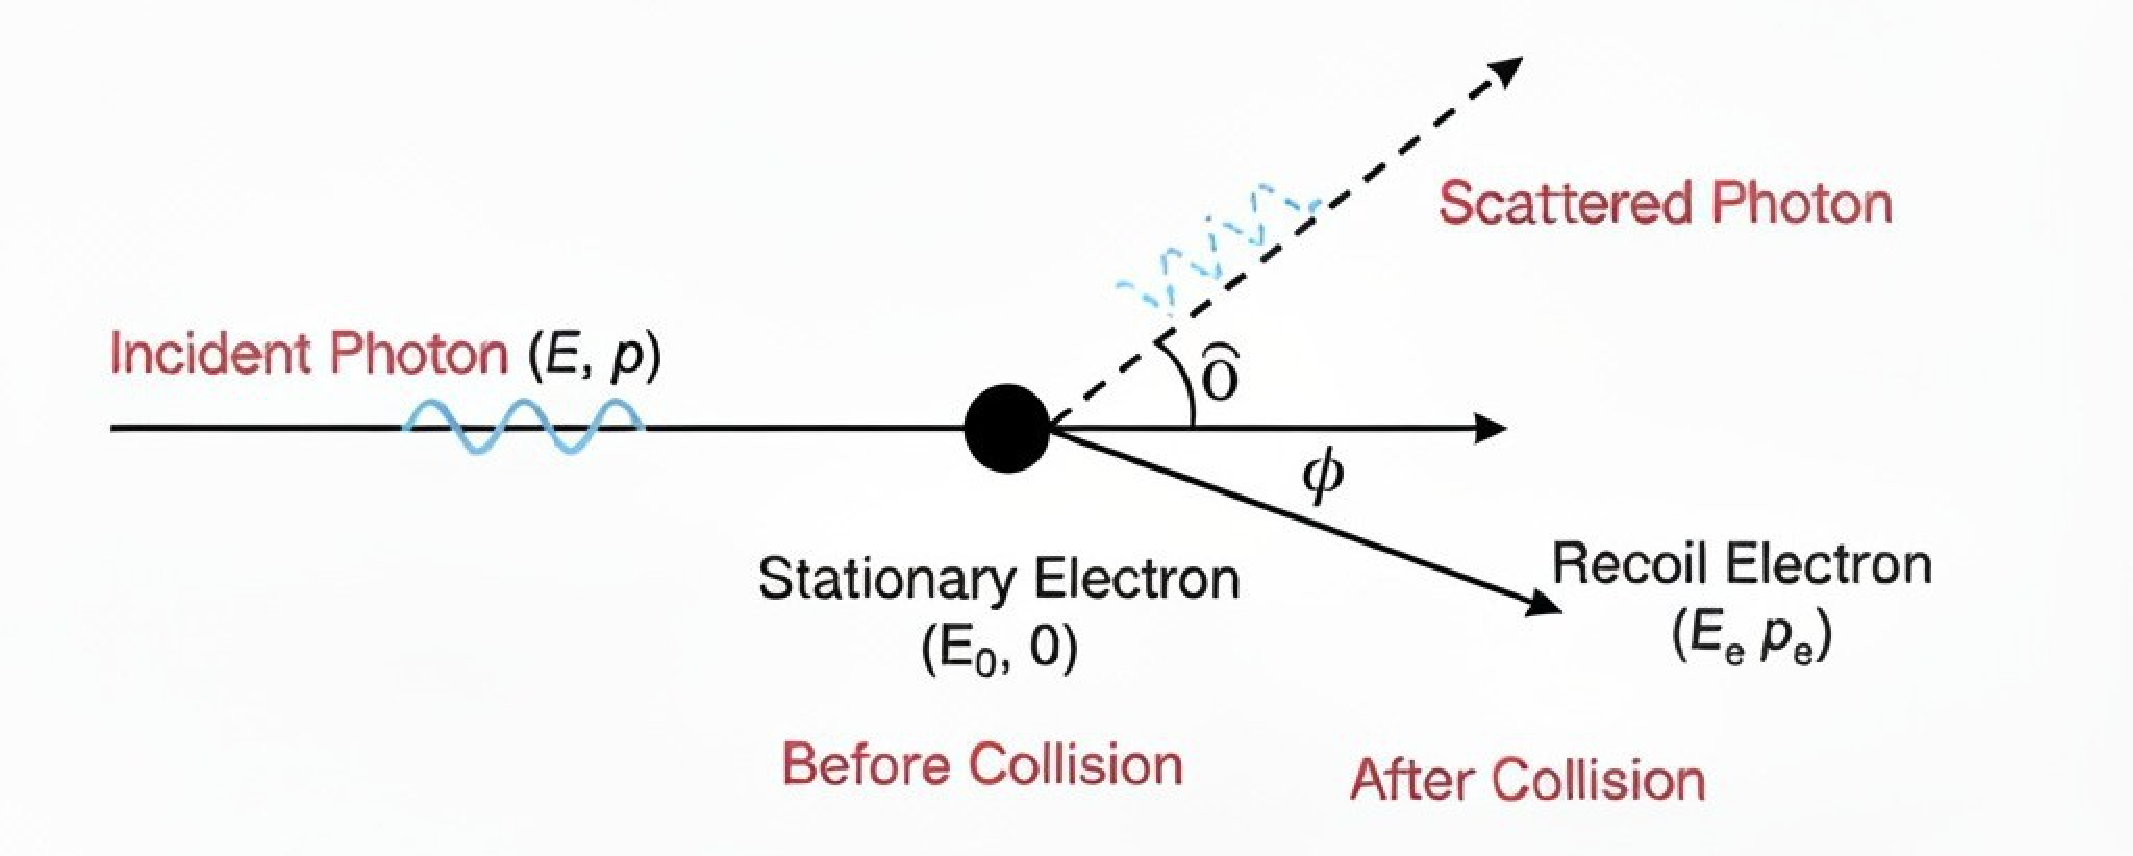
\includegraphics[width=0.5\textwidth]{imgs/ComptonScattering.pdf}
    \refstepcounter{figure}\label{fig:compton}
    \par\small \figurename~\thefigure:康普顿散射
\end{minipage}

\end{example}

\subsection{相对论动力学}
在相对论中,力的定义需要被修正以保持洛伦兹协变性。牛顿第二定律 $\bm{F} = m\bm{a}$ 不再适用。正确的形式是:
\begin{equation}
\bm{F} = \frac{\mathrm{d}\bm{p}}{\mathrm{d}t}
\end{equation}
其中 $\bm{p} = \gamma_u m_0 \bm{u}$ 是相对论动量。
这个力 $\bm{F}$ 不是一个四维矢量的空间部分,因此它在洛伦兹变换下的行为很复杂。
\begin{theorem}[功能关系]
力 $\bm{F}$ 所做的功等于物体动能的增加量 $\Delta E_k$。
\begin{equation}
\int \bm{F} \cdot \mathrm{d}\bm{s} = \Delta E_k
\end{equation}
\begin{proof}
\begin{equation}
\int \bm{F} \cdot \mathrm{d}\bm{s} = \int \frac{\mathrm{d}\bm{p}}{\mathrm{d}t} \cdot \bm{u}\mathrm{d}t = \int \bm{u} \cdot \mathrm{d}\bm{p}
\end{equation}
其中 $\bm{p} = m_0\bm{u}/\sqrt{1-u^2/c^2}$。
我们有 $\mathrm{d}\bm{p} = \mathrm{d}(\gamma_u m_0 \bm{u}) = m_0(\mathrm{d}\gamma_u \bm{u} + \gamma_u \mathrm{d}\bm{u})$。
因此 $\bm{u}\cdot\mathrm{d}\bm{p} = m_0(\gamma_u \bm{u}\cdot\mathrm{d}\bm{u} + u^2\mathrm{d}\gamma_u)$。
又因为 $\mathrm{d}(\gamma_u) = \gamma_u^3 (u/c^2) \mathrm{d}u$ 和 $\bm{u}\cdot\mathrm{d}\bm{u} = u\mathrm{d}u$,
代入后得到 $\bm{u}\cdot\mathrm{d}\bm{p} = m_0 \gamma_u^3 u \mathrm{d}u = \mathrm{d}(m_0\gamma_u c^2) = \mathrm{d}E$。
所以 $\int \bm{u} \cdot \mathrm{d}\bm{p} = \Delta E = \Delta E_k$ (因为静止能量不变)。
从这个证明中,我们也可以得到功率的表达式:
\begin{equation}
\frac{\mathrm{d}E}{\mathrm{d}t} = \bm{u} \cdot \frac{\mathrm{d}\bm{p}}{\mathrm{d}t} = \bm{u} \cdot \bm{F}
\end{equation}
\end{proof}
\end{theorem}
\textbf{注意:} 牛顿第三定律在相对论中一般不成立,因为相互作用的传递需要时间(以光速传递),这破坏了作用与反作用力的“同时性”。

\begin{definition}[闵可夫斯基力]
为了得到一个协变的动力学方程,我们定义闵可夫斯基力(四维力) $K^{\mu}$:
\begin{equation}
K^{\mu} = \frac{\mathrm{d}p^{\mu}}{\mathrm{d}\tau}
\end{equation}
其中 $\tau$ 是固有时。
四维力的分量为 $K^{\mu} = \gamma_u (\frac{1}{c}\frac{\mathrm{d}E}{\mathrm{d}t}, \bm{F})$。其中 $\frac{\mathrm{d}E}{\mathrm{d}t} = \bm{u}\cdot\bm{F}$ 是功率。
\end{definition}

\subsection{相对论电动力学}
\subsubsection{电磁场张量}
电场 $\bm{E}$ 和磁场 $\bm{B}$ 在洛伦兹变换下会相互转化。它们不是独立的实体,而是统一的电磁场的不同表现。
\begin{theorem}[场变换]
在从 $S$ 系到 $S'$ 系的洛伦兹变换下($S'$ 相对 $S$ 以速度 $v$ 沿 $x$ 轴运动),电磁场分量的变换关系为:
\begin{equation}
\begin{cases} 
E'_x = E_x \\
E'_y = \gamma(E_y - vB_z) \\
E'_z = \gamma(E_z + vB_y)
\end{cases}
\quad \text{和} \quad
\begin{cases} 
B'_x = B_x \\
B'_y = \gamma(B_y + \frac{v}{c^2}E_z) \\
B'_z = \gamma(B_z - \frac{v}{c^2}E_y)
\end{cases}
\end{equation}
\end{theorem}
为了以一种洛伦兹协变的形式来描述电磁场,我们引入电磁场张量。
\begin{definition}[电磁场张量]
电磁场张量 $F^{\mu\nu}$ 是一个二阶反对称张量,其分量由电场和磁场的分量构成:
\begin{equation}
F^{\mu\nu} = 
\begin{pmatrix}
0 & -E_x/c & -E_y/c & -E_z/c \\
E_x/c & 0 & -B_z & B_y \\
E_y/c & B_z & 0 & -B_x \\
E_z/c & -B_y & B_x & 0
\end{pmatrix}
\end{equation}
其对偶张量 $G^{\mu\nu} = \frac{1}{2}\epsilon^{\mu\nu\rho\sigma}F_{\rho\sigma}$ 为:
\begin{equation}
G^{\mu\nu} = 
\begin{pmatrix}
0 & -B_x & -B_y & -B_z \\
B_x & 0 & E_z/c & -E_y/c \\
B_y & -E_z/c & 0 & E_x/c \\
B_z & E_y/c & -E_x/c & 0
\end{pmatrix}
\end{equation}
\end{definition}
电磁场张量 $F^{\mu\nu}$ 在洛伦兹变换下满足张量变换法则: $F^{\mu'\nu'} = \Lambda^{\mu'}_{\rho}\Lambda^{\nu'}_{\sigma}F^{\rho\sigma}$。

\subsubsection{协变形式的麦克斯韦方程组}
\begin{definition}[四维电流密度]
四维电流密度 $J^{\mu}$ 定义为:
\begin{equation}
J^{\mu} = (\rho c, \bm{j})
\end{equation}
其中 $\rho$ 是电荷密度,$\bm{j}$ 是电流密度。电荷守恒定律(连续性方程)$\nabla\cdot\bm{j} + \frac{\partial\rho}{\partial t} = 0$ 可以用协变形式写为:
\begin{equation}
\partial_{\mu}J^{\mu} = 0
\end{equation}
其中 $\partial_{\mu} = \frac{\partial}{\partial x^{\mu}} = (\frac{1}{c}\frac{\partial}{\partial t}, \nabla)$。
\end{definition}
\begin{theorem}[协变形式的麦克斯韦方程组]
麦克斯韦方程组可以简洁地写成两个协变方程:
\begin{equation}
\partial_{\mu}F^{\mu\nu} = \mu_0 J^{\nu} \quad (\text{对应高斯定律和安培-麦克斯韦定律})
\end{equation}
\begin{equation}
\partial_{\mu}G^{\mu\nu} = 0 \quad (\text{对应高斯磁定律和法拉第感应定律})
\end{equation}
\end{theorem}

\subsubsection{洛伦兹力}
运动电荷在电磁场中受到的洛伦兹力可以用协变形式表示。
\begin{theorem}[协变洛伦兹力]
电荷为 $q$ 的粒子所受到的闵可夫斯基力 $K^{\mu}$ 为:
\begin{equation}
K^{\mu} = q F^{\mu\nu}U_{\nu}
\end{equation}
其中 $U_{\nu}$ 是粒子的四维速度。
这个方程的 $\mu=0$ 分量描述了电场对粒子做功的功率:
\begin{equation}
K^0 = \gamma_u \frac{\bm{u}\cdot\bm{F}}{c} = \gamma_u q \bm{u}\cdot\bm{E} / c
\end{equation}
其空间分量 ($\mu=1,2,3$) 描述了三维洛伦兹力:
\begin{equation}
\bm{K} = \gamma_u \bm{F} = \gamma_u q(\bm{E} + \bm{u} \times \bm{B})
\end{equation}
\end{theorem}

\subsection{电磁势和规范变换}
\begin{definition}[四维势]
电磁场可以通过电磁势来描述。我们定义四维势 $A^{\mu}$:
\begin{equation}
A^{\mu} = (\phi/c, \bm{A})
\end{equation}
其中 $\phi$ 是电标势,$\bm{A}$ 是磁矢势。
电磁场张量可以用四维势表示为:
\begin{equation}
F^{\mu\nu} = \partial^{\mu}A^{\nu} - \partial^{\nu}A^{\mu}
\end{equation}
\end{definition}
在洛伦兹规范 $\partial_{\mu}A^{\mu} = 0$ 下,麦克斯韦方程组可以简化为非齐次的波动方程:
\begin{equation}
\Box A^{\mu} = \mu_0 J^{\mu}
\end{equation}
其中 $\Box = \partial_{\mu}\partial^{\mu} = \frac{1}{c^2}\frac{\partial^2}{\partial t^2} - \nabla^2$ 是达朗贝尔算符。

最后,电流密度、电磁势和电磁场张量三者之间的关系可以总结为:
\begin{equation}
\begin{cases}
J^{\mu} \xrightarrow{\Box A^{\mu} = \mu_0 J^{\mu}} A^{\mu} \xrightarrow{F^{\mu\nu} = \partial^{\mu}A^{\nu} - \partial^{\nu}A^{\mu}} F^{\mu\nu} \\
\text{同时满足洛伦兹规范 } \partial_{\mu}A^{\mu} = 0
\end{cases}
\end{equation}

\begin{definition}[四维波矢]
电磁波的相位 $\Phi$ 是一个洛伦兹标量。对于平面波,$\Phi = \bm{k}\cdot\bm{r} - \omega t$。为了使其形式协变,我们定义四维波矢 $k^{\mu}$:
\begin{equation}
k^{\mu} = (\omega/c, \bm{k})
\end{equation}
这样相位可以写成 $k_{\mu}x^{\mu}$。光速不变原理要求 $k_{\mu}k^{\mu} = 0$,即 $(\omega/c)^2 - k^2 = 0$。
\end{definition}

\subsubsection{相对论多普勒效应和光行差}
通过对四维波矢 $k^{\mu}$ 进行洛伦兹变换,我们可以推导出光的频率和传播方向在不同惯性系下的变换关系,即相对论多普勒效应和光行差。
考虑一个光源在 $S$ 系中发出一束光,其角频率为 $\omega$,波矢为 $\bm{k}$。光的传播方向与 $x$ 轴的夹角为 $\theta$。因此 $k_x = (\omega/c)\cos\theta$,$k_y = (\omega/c)\sin\theta$ (为简单起见,设光在 $xy$ 平面内传播)。四维波矢为:
\begin{equation}
k^{\mu} = (\omega/c, (\omega/c)\cos\theta, (\omega/c)\sin\theta, 0)
\end{equation}
在相对于 $S$ 系以速度 $v$ 沿 $x$ 轴正方向运动的 $S'$ 系中,观测到的四维波矢为 $k^{\mu'}$。根据洛伦兹变换:
\begin{equation}
\begin{cases}
k^{0'} = \omega'/c = \gamma(k^0 - \beta k^1) = \gamma(\omega/c - \beta(\omega/c)\cos\theta) \\
k^{1'} = (\omega'/c)\cos\theta' = \gamma(k^1 - \beta k^0) = \gamma((\omega/c)\cos\theta - \beta\omega/c) \\
k^{2'} = (\omega'/c)\sin\theta' = k^2 = (\omega/c)\sin\theta
\end{cases}
\end{equation}

\begin{theorem}[相对论多普勒效应]
从第一个变换方程,我们可以直接得到两个参考系中频率的关系:
\begin{equation}
\omega' = \gamma\omega(1 - \beta\cos\theta) = \frac{1 - (v/c)\cos\theta}{\sqrt{1 - v^2/c^2}}\omega
\end{equation}
这就是相对论多普勒效应的普适公式。它包含了两个经典物理中不存在的效应:
\begin{itemize}
    \item \textbf{横向多普勒效应}: 即使在光源的运动方向与观测方向垂直时(在 $S$ 系中,$\theta=\pi/2$),频率也会发生改变。
    \begin{equation}
    \omega' = \gamma\omega = \frac{\omega}{\sqrt{1 - v^2/c^2}} \quad (\text{当 } \theta = \pi/2)
    \end{equation}
    这是一个纯粹的相对论效应,来源于时间膨胀。观察者会认为运动时钟(光源的振荡周期)变慢了,因此观测到的频率变高了。
    \item \textbf{纵向多普勒效应}: 当光源沿观测方向运动时。
    \begin{itemize}
        \item 光源远离观察者 ($\theta = 0$): $\omega' = \omega\sqrt{\frac{1-\beta}{1+\beta}}$。频率降低(红移)。
        \item 光源朝向观察者 ($\theta = \pi$): $\omega' = \omega\sqrt{\frac{1+\beta}{1-\beta}}$。频率升高(蓝移)。
    \end{itemize}
\end{itemize}
\end{theorem}

\begin{theorem}[光行差]
光行差描述的是光的传播方向因相对运动而发生的改变。我们可以通过将 $k^{1'}$ 和 $k^{2'}$ 的变换式相除来得到 $\theta$ 和 $\theta'$ 的关系。
\begin{equation}
\tan\theta' = \frac{k^{2'}}{k^{1'}} = \frac{(\omega/c)\sin\theta}{\gamma((\omega/c)\cos\theta - \beta\omega/c)} = \frac{\sin\theta}{\gamma(\cos\theta - \beta)}
\end{equation}
为了得到更常用的形式,我们使用逆变换(将 $\beta$ 换为 $-\beta$,并交换带撇和不带撇的变量),可以得到:
\begin{equation}
\cos\theta = \frac{\cos\theta' + \beta}{1 + \beta\cos\theta'}
\end{equation}
这个公式描述了在 $S'$ 系中以 $\theta'$ 角传播的光,在 $S$ 系中被观测到的传播方向 $\theta$。例如,从天顶 ($\theta'=\pi/2$) 射来的一束星光,在运动的地球 ($S$ 系) 上看来,将偏向运动的前方,即 $\cos\theta = \beta > 0$。
\end{theorem}

\end{document}